

%% La classe stageM2R s'appuie sur la classe memoir, plus d'information sur le paquet: http://www.ctan.org/pkg/memoir
%% option possible de la classe stageM2R
% utf8  -> encodage du texte UTF8 (défaut: Latin1)
% final -> mode rapport de stage final (défaut: mode étude bibliographique)
% private -> indique une soutenance privée (défaut: soutenance publique)
% \documentclass[utf8]{stageM2R} %-> etude bibliographique
\documentclass[utf8,final]{stageM2R} %-> rapport final

\usepackage{wrapfig}
\usepackage{hhline}
\usepackage{subcaption}
\usepackage[]{algorithm2e}
\usepackage{amsthm}
\usepackage{mathtools}
\usepackage{float}
\usepackage{tikz}
\usepackage{tikz-qtree}
\usepackage{csquotes}
\usepackage{indentfirst}
\usepackage{upgreek}
\usepackage{slashbox}
\usepackage{forest}
\usepackage{hyperref}
\usepackage{pbox}
\usetikzlibrary{trees}
\usetikzlibrary{babel}
\usetikzlibrary{arrows,automata,positioning}

\usepackage[
    maxbibnames=9,
    maxnames=2,
    % style=nature,
    % citestyle=mla,
    backend=bibtex]
{biblatex}

\DeclareCiteCommand{\citeauthornsc}
  {\renewcommand*{\mkbibnamelast}[1]{####1}%
   \boolfalse{citetracker}%
   \boolfalse{pagetracker}%
   \usebibmacro{prenote}}
  {\ifciteindex
     {\indexnames{labelname}}
     {}%
   \printnames{labelname}}
  {\multicitedelim}
  {\usebibmacro{postnote}}

\DeclareCiteCommand*{\citeauthornsc}
  {\renewcommand*{\mkbibnamelast}[1]{####1}%
   \boolfalse{citetracker}%
   \boolfalse{pagetracker}%
   \usebibmacro{prenote}}
  {\ifciteindex
     {\indexnames{labelname}}
     {}%
   \printnames[][1-1]{labelname}}
  {\multicitedelim}
  {\usebibmacro{postnote}}



\bibliography{biblio.bib}

% \newcommand*{\addheight}[2][.5ex]{%
%   \raisebox{0pt}[\dimexpr\height+(#1)\relax]{#2}%
% }

%%%%%%%%%%%%%%%%%%%%%%%%%%%%
%%% Déclaration du stage %%%
%%%%%%%%%%%%%%%%%%%%%%%%%%%%

%% auteur
\author{Noé Le Philippe}
%% encadrants
\supervisors{William Puech \\ Christophe Fiorio}
%% lieu du stage (Optionnel)
\location{Équipe ICAR - LIRMM UMR 5506 - CNRS, Université de Montpellier}
%% titre du stage
\title{La phylogénie des images dans les réseaux sociaux} 
%% parcours du master
\track{IMAGINA}  
%% date de soutenance (Optionnel)
% \date{\today} 
%% version du rapport (Optionnel)
% \version{1}
%% Résumé en francais
\abstractfr{
  Il est aujourd'hui extrêmement facile de manipuler des images et de les partager à l'aide des réseaux sociaux. Il est important d'identifier l'historique des transformations appliquées aux images afin de leur accorder un minimum crédibilité. Dans le cadre de ce stage, l'objectif principal de nos recherches consiste à calculer l'arbre de phylogénie d'un ensemble d'images où les images sont issues de différentes compressions JPEG successives. À chaque étape, une image enfant est donc créée à partir de la compression d'une image parent. Dans ce rapport nous présentons dans l'état de l'art les différentes méthodes de reconstruction d'un arbre phylogénétique et traitons de la détection et de l'identification des compressions JPEG multiples. Nous présentons également notre méthode qui s'articule autour d'un point central : la décision binaire entre deux images et nous détaillons les résultats obtenus grâce à cette méthode. 
% approche un théorème permettant de réduire le calcul de l'arbre à une décision binaire entre deux images et un algorithme de reconstruction d'arbre.

\vspace{5mm}
\textbf{Mots clés.} Phylogénie des images, JPEG, Compressions multiples, Arbre de phylogénie

}
%% Résumé en anglais
\abstracteng{
  Nowadays it is extremely easy to tamper images and share them thanks to social media. Identifying the tamper history is mandatory to be able to trust any of those images. During this internship, our main goal is to compute the image phylogeny tree of an image set, where images are created from successive JPEG compressions. Every step, a child image is created from the compression of a parent image. In this master's thesis we present in a state of the art several methods for computing the image phylogeny tree and take an overview of the different methods for detecting and identifying multiple JPEG compressions. We also introduce our method based on a binary decision between two images and explain the results obtained with this method.
% approach with a theorem that allows us to reduce the image phylogeny tree estimation to a binary decision between two images and we describe a tree building algorithm.

\vspace{5mm}
\textbf{Mots clés.} Image phylogeny, JPEG, Multiple compressions, Phylogeny tree

}



\begin{document}   
%\selectlanguage{english} %% --> turn the document into english mode (Default is french)
\selectlanguage{french} 
\frontmatter  %% -> pas de numérotation numérique
\maketitle    %% -> création de la page de garde et des résumés
\cleardoublepage   
\tableofcontents %% -> table des matières
\mainmatter  %% -> numérotation numérique


%%%%%%%%%%%%%%%%%%%%%%%%%%%%%%
%%%%   DEBUT DU RAPPORT   %%%%
%%%%%%%%%%%%%%%%%%%%%%%%%%%%%%

\chapter{Introduction}
La phylogénie, en sciences naturelles, est définie comme l'étude des relations de parenté entre êtres vivants. Et c'est exactement de cela qu'il s'agit dans le cas des images, l'étude des relations de parenté entre images. \autocite{phylogeny} \\
À l'ère du numérique et des réseaux sociaux, il n'a jamais été aussi simple de partager des idées et du contenu. À chaque partage cependant, l'information peut être modifiée plus ou moins fortement. Les images, puisque c'est là notre sujet d'étude, peuvent avoir subi un certain nombre de transformations et de modifications avant d'être publiées sur les réseaux sociaux. C'est dans ce contexte que nous allons intervenir afin de tenter de reconstituer la phylogénie d'une image. Il peut être difficile de différentier une image modifiée de l'originale, et de savoir laquelle est l'originale alors que cette détection est cruciale, surtout dans un monde où l'information peut être facilement falsifiée par tout un chacun. Les applications sont multiples et variées, et ne se cantonnent pas à la détection et la discrimination d'images altérées. Il est également possible de se servir de la phylogénie des images pour optimiser l'espace de stockage en ne gardant que l'image originale et l'historique des modifications ou encore suivre la diffusion et l'évolution des idées sur les réseaux sociaux. 

Dans ce chapitre nous commencerons par définir ce que sont les near-duplicate images, puis nous détaillerons la notion d'arbre phylogénétique et enfin nous expliquerons pourquoi nous nous sommes restreints à la compression JPEG dans le cadre de cette étude. Nous ferons un état de l'art dans le chapitre \ref{chap2} où nous présenterons les différentes approches pour calculer l'arbre de phylogénie. Nous aborderons également la problématique de la détection des recompressions et l'estimation du nombre de recompressions. Nous présentons ensuite notre méthode dans le chapitre \ref{chap3}, où détaillerons en quoi consiste, et comment est prise une décision binaire entre deux images, et comment l'arbre est ensuite reconstruit. Les résultats obtenus grâce à cette méthode seront ensuite présentés et expliqués chapitre \ref{chap4} puis nous finirons par conclure chapitre \ref{chap5}.

 % un algorithme de reconstruction d'arbre sera détaillé, en plus du théorème qui sera la base de la suite du stage. Nous finirons par conclure dans le chapitre \ref{chap4}.
\newpage

\section{Near-duplicate images (NDI)}
\label{subsec:ndi}
Nous travaillons sur un ensemble d'images, toutes similaires visuellement, et au milieu de cet ensemble d'images, nous devons décider quelle image est le parent de quelle autre, ou autrement dit, quelles images sont des \textbf{near-duplicates}. \citeauthornsc{joly2007content} \autocite{joly2007content} définissent la notion de near-duplicate comme suit : $I_{n+1} = T(I_{n}), T \in \mathcal{T}$ où $I_{n}$ est l'image parent, $I_{n+1}$ est l'image à la génération suivante $n+1$, l'image enfant et $\mathcal{T}$ est un ensemble de transformations autorisées, $I_{n+1}$ et $I_{n}$ sont alors des NDI. Dans le cas général, $\mathcal{T} = $ \textit{\{resampling, cropping, affine warping, color changing, lossy compression\}}. La figure \ref{fig:near-duplicates-images} montre un exemple de near-duplicates. Le \textit{resampling}, ou rééchantillonage en français revient à changer le nombre de pixels de l'image, le \textit{crop} est illustré figure \ref{lena-crop}, \textit{affine warping} englobe tout ce qui peut être translation ou rotation, \textit{color changing} concerne tout ce qui va changer la couleur, comme le changement de contraste par exemple, ou le passage au noir et blanc (figure \ref{lena-bw}), et enfin \textit{lossy compression} est la compression avec pertes, une dégradation de l'image pour réduire son poids.
% , dans le cadre de ce stage cependant, $\mathcal{T} = $ \textit{\{lossy compression\}}. 
Notons l'utilisation du terme \textit{transformations autorisées}. Ce terme est double, d'une part, il place une limite arbitraire dans la force de la transformation, par exemple une image croppée à plus de 10\% pourra ne pas pas être considérée comme un near-duplicate, et d'autre part, il permet de restreindre l'espace des transformations possibles. 
% Ainsi, dans le cadre du stage, seules les images de la troisième case de Fig. \ref{fig:near-duplicates-images} seront des NDI.
Ces transformations peuvent évidemment se composer, et une image enfant peut être le résultat de plusieurs transformations.


\vspace{5mm}
\textbf{Note.} \textit{Nous utiliserons les notions relation parent-enfant et relation de parenté de manière interchangeable dans le reste de ce rapport, mais c'est bien d'une relation parent-enfant qu'il s'agit.}

\begin{center}
  \begin{figure}[H]
    \begin{subfigure}{.33\textwidth}
      \centering
      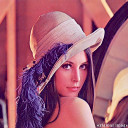
\includegraphics[width=23mm]{images/lena_base.jpg} 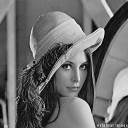
\includegraphics[width=23mm]{images/lena_bw.jpg}
      \caption{couleur $\to$ noir et blanc}
      \label{lena-bw}
    \end{subfigure}
    \begin{subfigure}{.33\textwidth}
      \centering
      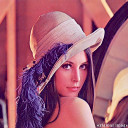
\includegraphics[width=23mm]{images/lena_base.jpg} 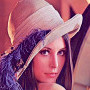
\includegraphics[width=23mm]{images/lena_crop.jpg}
      \caption{image entière $\to$ image croppée}
      \label{lena-crop}
    \end{subfigure}
    \begin{subfigure}{.33\textwidth}
      \centering
      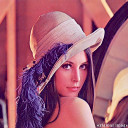
\includegraphics[width=23mm]{images/lena_base.jpg} 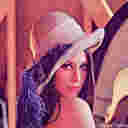
\includegraphics[width=23mm]{images/lena_comp.jpg}
      \caption{image $\to$ image compressée}
      \label{lena-comp}
    \end{subfigure}
    \caption{Exemple de near-duplicates}
    \label{fig:near-duplicates-images}
  \end{figure}
\end{center}

\section{Arbre phylogénétique (Image Phylogeny Tree - IPT)}
\label{ipt}
L'arbre phylogénétique (IPT) est l'arbre représentant les relations de parenté entre les différentes images. Il est extrait d'un ensemble de NDI, et constitue l'objectif final de l'application. La figure \ref{fig:set-to-tree} illustre la construction de l'IPT à partir d'un ensemble de NDI. Le passage d'une génération à l'autre, autrement dit d'un noeud à son fils, se fait à travers la transformation $I_{n+1} = T(I_{n})$, ainsi, une image $I_{n+1}$ et son parent $I_{n}$ sont des NDI, alors qu'une image $I_{n+1,i}$ et sa soeur $I_{n+1,j}$, $i \neq j$ ne le sont pas (figure \ref{fig:tree-extract}).

La reconstruction de l'arbre se concentre autour de deux problèmes principaux. Le premier est l'identification de la racine ($n=0$), et le second est l'estimation du reste de l'arbre, et en particulier positionner précisément chacune des images dans leur génération respective (valeur de $n$). Il est en effet critique d'identifier correctement la racine. Prenons par exemple un des cas d'utilisation de l'IPT, la détection d'altération d'images. L'idée est que pour un ensemble d'images, plus la génération est proche de la racine, c'est à dire plus $n$ est petit, moins l'image a subi de transformations, et donc moins elle est altérée. Avec comme cas particulier $n = 0$, l'image est alors la génération $0$ : la racine. Notons que si la racine est mal identifiée, une image pourra être à tort marquée comme altérée.
% Nous déduirons, à tort, qu'une image n'a pas été altérée. 
Il n'est pas toujours garanti que la totalité des images de l'arbre original soit présente, l'identification précise de la génération peut alors se révéler complexe. Certaines transformations peuvent être mineures, et difficile à détecter, dans ce cas deux images de deux générations proches $n$ et $n+k$, avec $k$ petit ($k = 1, 2$ ou 3 par exemple), peuvent être identifiées à tort comme appartenant à la même génération. En conclusion, il est clair que l'arbre ne sera qu'une estimation, et sauf dans des cas idéaux, ne sera pas l'arbre original.

\begin{figure}
  \begin{center}
    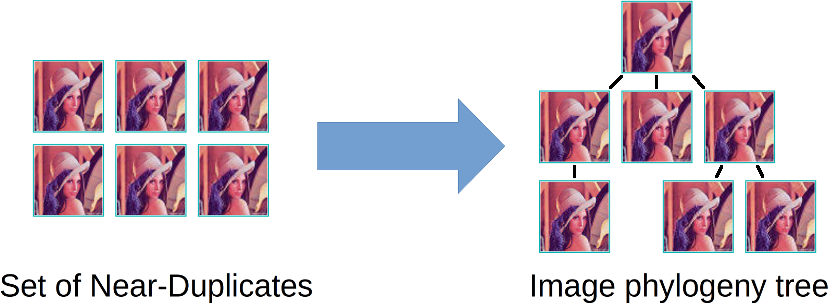
\includegraphics[width=120mm]{images/set_to_tree}
    \caption{Passage d'un ensemble de NDI à un arbre phylogénétique}
    \label{fig:set-to-tree}
  \end{center}
\end{figure}

\begin{figure}
  \begin{center}
    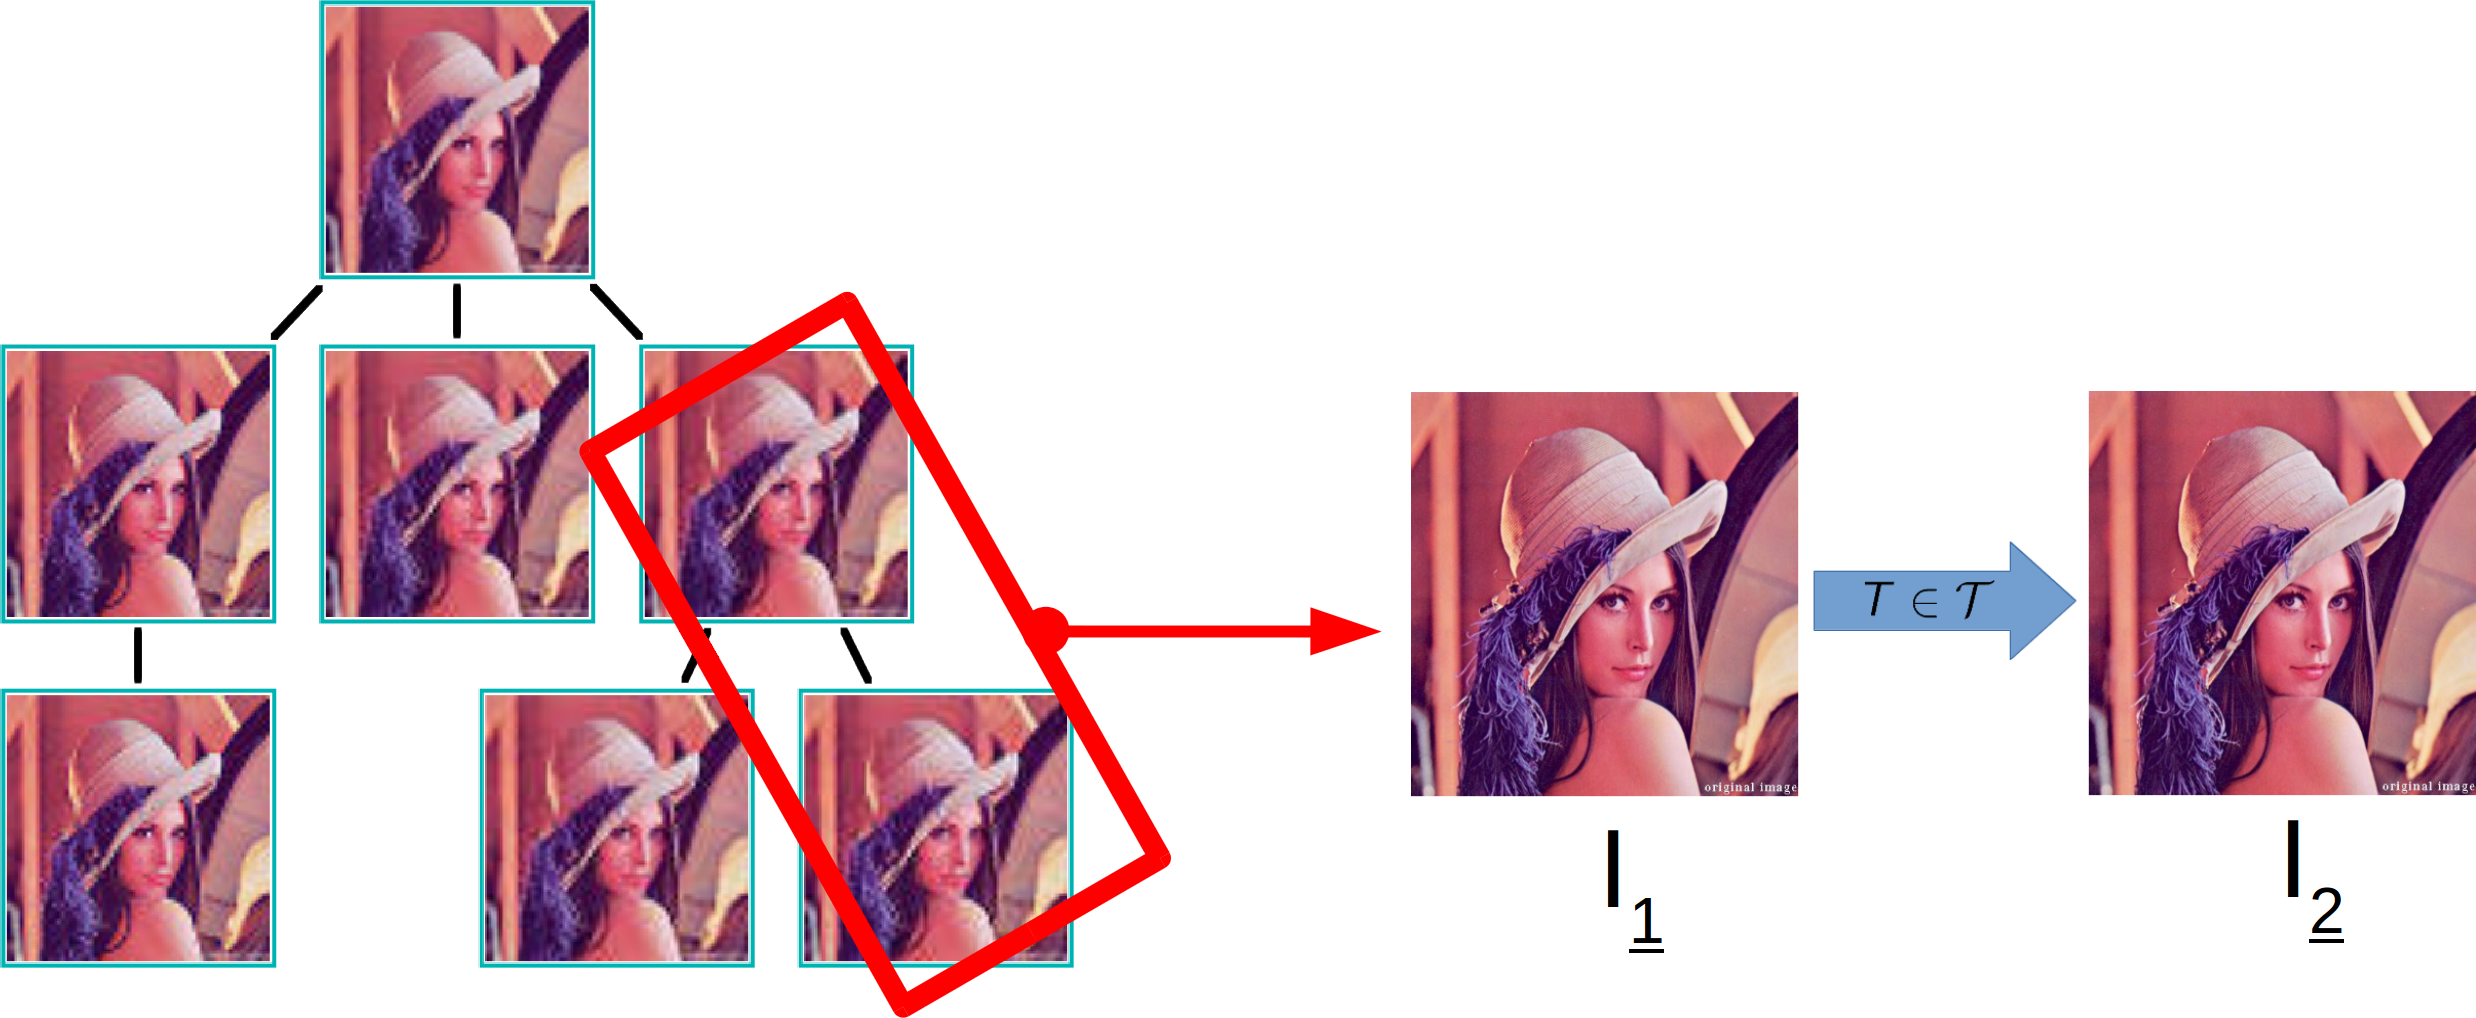
\includegraphics[width=120mm]{images/tree_extract}
    \caption{Passage d'une image parent à l'image enfant}
    \label{fig:tree-extract}
  \end{center}
\end{figure}

\section{Pourquoi se restreindre à la compression comme transformation ?}
Dans le cadre du stage, nous proposons de réduire l'espace des transformations à $\mathcal{T} =$ \textit{\{lossy compression\}} avec JPEG comme algorithme de compression. L'étude et la détection des recompressions JPEG est en effet un sujet suffisamment vaste et complexe pour que cela soit la seule transformation étudiée dans le cadre de ce stage de recherche. C'est de plus un sujet qui à notre connaissance n'a pas été traité dans le cadre de la phylogénie des images, et qui est largement étudié dans le domaine du forensics (criminalistique en français). L'étude et la détection des recompressions est en effet un sujet vaste, la figure \ref{comp_vaste} détaille l'étendue du problème. La compression JPEG sera détaillée dans le chapitre \ref{chap2} en section~\ref{detail_jpeg}. Aussi la seule caractéristique dont nous parlerons dans cette section est le facteur de qualité $Q$. $Q \in [1..100]$ et plus $Q$ est grand, plus l'image sera de bonne qualité, mais moins elle sera compressée. Nous sommes donc en présence de trois cas pour les recompressions successives : le premier est le cas où tous les $Q$ successifs sont égaux, dans le second cas, l'image est plus dégradée à chaque recompression, et dans le troisième, nous n'avons aucune idée sur la manière dont l'image a été recompressée par rapport à son parent. Elle peut avoir été recompressée avec la même qualité, ou une meilleure qualité, ou encore une moins bonne qualité.

  \begin{figure}[H]
    \begin{center}
      % \begin{tikzpicture}[auto, distance=2in,sibling distance=.25in]
      \scalebox{0.85}{%
      \begin{tikzpicture}[auto,node distance=2.8cm]

        \tikzstyle{every state}=[shape=rectangle,minimum width=1.3in,text width=1.3in, align=center,fill=blue!30]

        \node[draw=none,fill=none] (A) {image originale};
        \node[state] (B) [right=0.7cm of A] {première compression JPEG avec $Q_{1}$};
        \node[draw=none,fill=none,minimum width=1.1in,text width=1.1in] (C) [right=0.7cm of B] {première image compressée};
        \node[state] (D) [above right=1.7cm and 0.9cm of C] {$n^{ieme}$ compression JPEG avec $Q_{n+1} = Q_{n}$};
        \node[state] (E) [right=0.9cm of C] {$n^{ieme}$ compression JPEG avec $Q_{n+1} < Q_{n}$};
        \node[state] (F) [below right=1.7cm and 0.9cm of C] {$n^{ieme}$ compression JPEG avec $Q_{n+1}\ \{<,>,=\}\ Q_{n}$};
        \node[draw=none,fill=none,minimum width=0.79in,text width=0.79in] (G) [right=0.7cm of D] {$n^{ieme}$ image compressée};
        \node[draw=none,fill=none,minimum width=0.79in,text width=0.79in] (H) [right=0.7cm of E] {$n^{ieme}$ image compressée};
        \node[draw=none,fill=none,minimum width=0.79in,text width=0.79in] (I) [right=0.7cm of F] {$n^{ieme}$ image compressée};

        \node[draw=none,fill=none] (D1) [below=0.7cm of D] {};
        \node[draw=none,fill=none] (D2) [below=0.94cm of G] {};

        \node[draw=none,fill=none] (E1) [below=0.7cm of E] {};
        \node[draw=none,fill=none] (E2) [below=0.94cm of H] {};

        \node[draw=none,fill=none] (F1) [below=0.7cm of F] {};
        \node[draw=none,fill=none] (F2) [below=0.94cm of I] {};

        
        \path [->] (A) edge node[left] {} (B);
        \path [->] (B) edge node[left] {} (C);      
        \path [->] (C.east) edge node[left] {} (D.west);
        \path [->] (C.east) edge node[left] {} (E.west);
        \path [->] (C.east) edge node[left] {} (F.west);
        \path [->] (D) edge node[left] {} (G);
        \path [->] (E) edge node[left] {} (H);
        \path [->] (F) edge node[left] {} (I);

        \path [->] (D1.center) edge node[left] {} (D);
        \path [-] (D2.center) edge node[left] {} (D1.center);
        \path [-] (G.south) edge node[left] {} (D2.center);

        \path [->] (E1.center) edge node[left] {} (E);
        \path [-] (E2.center) edge node[left] {} (E1.center);
        \path [-] (H.south) edge node[left] {} (E2.center);

        \path [->] (F1.center) edge node[left] {} (F);
        \path [-] (F2.center) edge node[left] {} (F1.center);
        \path [-] (I.south) edge node[left] {} (F2.center);
      \end{tikzpicture}}
      \caption{Exemple des différents scénarios de recompression d'images}
      \label{comp_vaste}
    \end{center}
  \end{figure}

Nous avons choisi de nous concentrer particulièrement sur le deuxième cas, lorsque le facteur de qualité du parent est strictement supérieur à celui de l'enfant.

\chapter{État de l'art}
\label{chap2}
Ce chapitre tentera de faire un état de l'art des différentes techniques de calcul d'un arbre phylogénétique, puis traitera des différentes méthodes permettant d'extraire des informations de plusieurs compressions successives, et enfin présentera quelques calculs de distances.
\section{Étude de l'arbre phylogénétique}
\label{etude}
\subsection{La Visual Migration Map (VMM)}
L'article de \citeauthornsc{kennedy2008internet} est à notre connaissance le premier article concernant vraiment notre sujet \autocite{kennedy2008internet}. Les auteurs proposent une approche permettant de détecter automatiquement la manière dont une image a été éditée ou manipulée, et d'en extraire des relations parent-enfant entre les images. Il vont construire à partir le l'estimation de ces transformations une Visual Migration Map (VMM) (voir figure \ref{vmm}) qui est en fait un arbre de phylogénie.

\citeauthornsc{kennedy2008internet} partent du principe que les transformations sont directionnelles, c'est à dire qu'il n'est possible d'aller que d'une image moins transformée vers une image plus transformée. Ainsi, ils vont tenter d'estimer la direction de chaque transformation entre deux images $I_{1}$ et $I_{2}$ (sachant que $\mathcal{T}$ = \textit{\{scaling, cropping, grayscale, overlay, insertion\}}). Trois scénarios sont alors possibles : si toutes les transformations sont dans le même sens, l'image fille est alors celle vers qui pointent les transformations, si les transformations sont dans des sens contraires, les images sont sûrement des soeurs, elles n'ont en tous cas pas de relation parent-enfant, et enfin si aucune transformation n'a été détectée, c'est que soit les images sont identiques, soit qu'elles ne sont pas des near-duplicates. La figure \ref{vmm-directionnel} illustre ce principe par un exemple.
\\ \indent
Un graphe est ensuite construit à partir des couples d'images pour lesquels une relation parent-enfant a été détectée. À noter qu'une relation parent-enfant ne veut pas forcément dire que c'est le parent direct mais plutôt un ancêtre. Ainsi, un noeud du graphe (une image) peut avoir plusieurs noeuds parents, pour finalement obtenir l'arbre désiré, seuls les chemins les plus longs sont conservés, comme on peut le voir figure \ref{vmm-tree}.

%%%%% parler de comment sont calculées les directions des transformations.
%%%%% parler des résultats ?
%%%%% parler de ce qui est bien dans cette méthode et de ce que l'on va utiliser.

% \begin{wrapfigure}{R}{0.5\textwidth}
%   \begin{center}
%     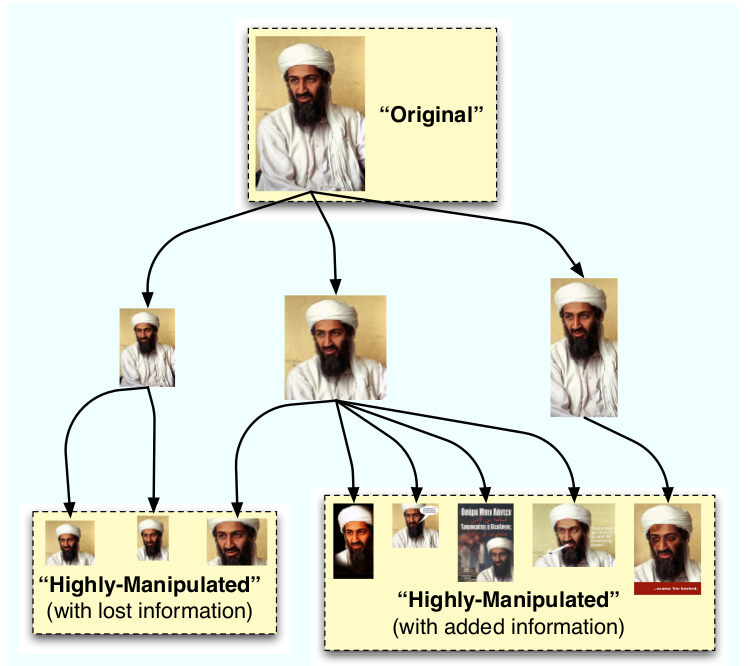
\includegraphics[width=0.48\textwidth]{images/vmm.png}
%   \end{center}
%     \label{vmm}
%     \caption{Exemple de VMM, tiré de \autocite{internet}}
% \end{wrapfigure}

\begin{figure}
  \begin{center}
    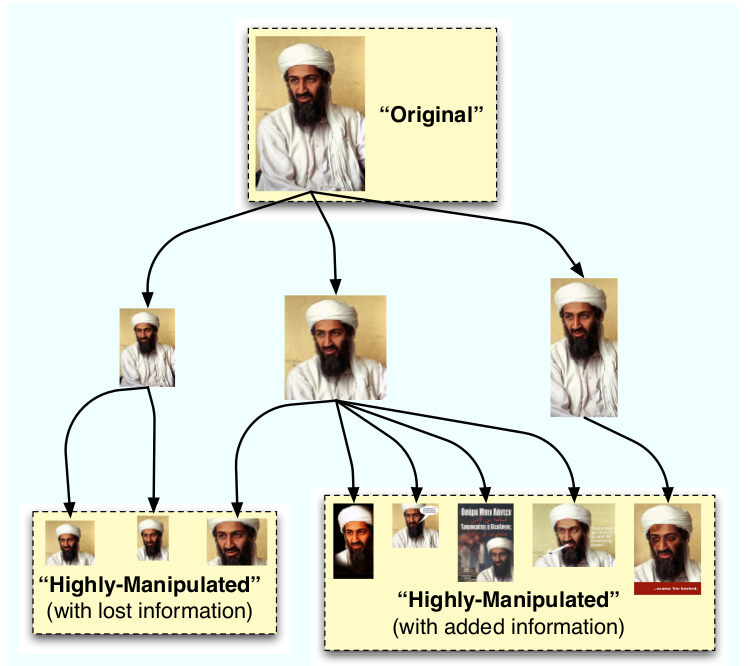
\includegraphics[width=70mm]{images/vmm.png}
    \caption{Exemple de VMM, issu de \autocite{kennedy2008internet}.}
    \label{vmm}
  \end{center}
\end{figure}

\begin{figure}
  \begin{center}
    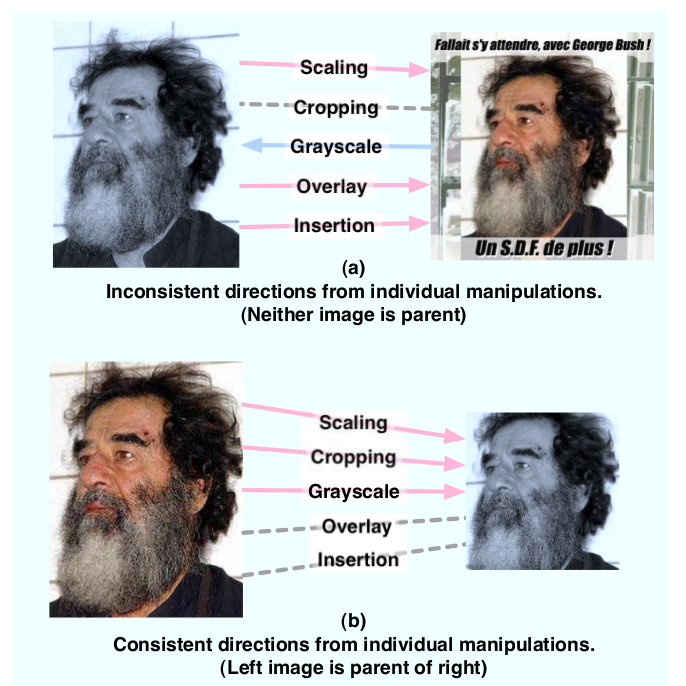
\includegraphics[width=70mm]{images/vmm_directionnel.png}
    \caption{Exemple de direction des transformations, issu de \autocite{kennedy2008internet}.}
    \label{vmm-directionnel}
  \end{center}
\end{figure}

\begin{figure}
  \begin{center}
    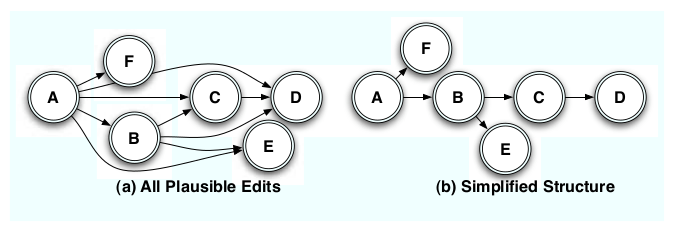
\includegraphics[width=100mm]{images/vmm_tree.png}
    \caption{Exemple de simplification de graphe, issu de \autocite{kennedy2008internet}.}
    \label{vmm-tree}
  \end{center}
\end{figure}

\subsection{Image Phylogeny Tree (IPT)}
\label{diasetal}

Tout comme l'approche présentée précédemment, \citeauthornsc{dias2010first} \autocite{dias2010first}\autocite{dias2012image} proposent une approche basée sur le contenu de l'image. Elle consiste a mapper une image sur le domaine d'une autre, pour pouvoir les comparer, et ensuite estimer le coût de cette opération. L'hypothèse est que si deux images sont dépendantes, alors il est possible d'obtenir l'une en appliquant une transformation à l'autre. 

Les images sont comparées à l'aide d'une fonction de dissimilarité, ou \textit{dissimilarity function d(.,.)} qui renvoie des petites valeurs lorsque les images sont proches (elles ont subi des transformations similaires). L'équation \ref{dissimilarity-function} détaille cette fonction. $I_{m}$ et $I_{n}$ sont les deux images qui vont être comparées, et $T_{\overrightarrow{\beta}} \in \mathcal{T}$ est la transformation en train d'être estimée, où $\overrightarrow{\beta}$ est l'ensemble des valeurs que peut prendre en paramètre la transformation. Dans le cas de la compression JPEG par exemple $\overrightarrow{\beta} = \{1..100\}$. La transformation la plus faible est gardée comme résultat, c'est la transformation la plus probable qu'a pu subir l'image. À noter que $d(.,.)$ est asymétrique, c'est à dire que $d(I_{m},I_{n}) \neq d(I_{n},I_{m})$, ce qui est parfaitement logique, en plus d'être nécessaire, sachant que les transformation sont directionnelles, comme expliqué précédemment.

\begin{equation}
  d(I_{m},I_{n}) = \underset{T_{\overrightarrow{\beta}}}{min}\left | I_{n} - T_{\overrightarrow{\beta}}(I_{m}) \right |_{comparison\ method}
  \label{dissimilarity-function}
\end{equation}

Nous voyons donc bien que la problématique principale de cette méthode est de trouver une bonne méthode de comparaison. Les auteurs procèdent de la manière suivante : 
\begin{enumerate}
  \item Trouver des points caractéristiques (SURF \autocite{bay2008speeded}),
  \item Filtrer les points et estimer les paramètres de transformation affines tels que les translations, rotations et rééchantillonages avec RANSAC \autocite{ransac},
  \item Calculer la moyenne et la variance de chaque canal couleur de $I_{n}$ pour normaliser les couleurs de $I_{m}$,
  \item Compresser les résultats des deux étapes précédentes avec la table de quantification de $I_{n}$
\end{enumerate}

La dissimilarité entre les deux images est enfin obtenue en utilisant la \textit{minimum mean squared error} (MMSE) entre les deux images dans le domaine spatial. (\textit{comparison method} de l'équation \ref{dissimilarity-function})

Ces quatre étapes servent à rendre les images comparables, en mappant l'une dans le domaine de l'autre, pour avoir des résultats pertinents.
%%%% Analyser leur méthode et ne pas simplement la décrire ?
% \vspace{3mm}
\paragraph{}

La distance $d(.,.)$ est donc appliquée à tous les couples d'images de l'ensemble, pour créer une matrice de dissimilarité, ou \textit{dissimilarity matrix}, une matrice de taille $n\times n$ qui sera ensuite donnée comme entrée à leur algorithme de reconstruction d'arbre, Oriented Kruskal. Cet algorithme est expliqué de manière exhaustive dans \autocite{dias2012image}. Dans le chapitre \ref{chap3}, nous proposons une approche différente, notre reconstruction sera donc également différente. 
 % et ayant une approche différente (chapitre \ref{chap:notre_approche}), la reconstruction sera également différente.
% \vspace{3mm}
\paragraph{}                    

En plus de proposer une approche pour reconstituer l'arbre de phylogénie, \citeauthornsc{dias2012image} proposent une approche pour comparer deux arbres, et donc évaluer notre arbre reconstruit s'il est comparé avec la vérité terrain. Il consiste en quatre métriques : \\
\renewcommand{\arraystretch}{2}
\begin{tabular}{ll}
  \textbf{Root} & $
                  R(IPT_{1}, IPT_{2}) = $
                  \scalebox{0.65}{%
                  $
                  \begin{cases}
                    1 & if\ \texttt{Root(IPT}_{1}) = \texttt{Root(IPT}_{2}) \\
                    0 & Otherwise
                  \end{cases}
                        $} \\
  \textbf{Edges} & $E(IPT_{1}, IPT_{2}) = \frac{|E_{1} \cap E_{2}|} {n - 1}$ \\
  \textbf{Leaves} & $L(IPT_{1}, IPT_{2}) = \frac{|L_{1} \cap L_{2}|} {|L_{1} \cup L_{2}|}$ \\
  \textbf{Ancestry} & $A(IPT_{1}, IPT_{2}) = \frac{|A_{1} \cap A_{2}|} {|A_{1} \cup A_{2}|}$
\end{tabular}
\renewcommand{\arraystretch}{1.}
% \vspace{5mm}
\paragraph{}

\textbf{Root} est triviale, et renvoie si les racines sont identiques. \textbf{Edges} mesure le ratio de noeuds ayant le bon parent, \textbf{Leaves} est le ratio de feuilles correctes, et enfin \textbf{Ancestry} est le ratio d'ancêtres corrects jusqu'à la racine.

Ces métriques serviront à évaluer nos résultats dans la suite du stage.

\section{Analyse des recompressions JPEG}
\label{detail_jpeg}
Notre but n'est pas vraiment de détecter si une image a été compressée plusieurs fois, nous sommes en effet quasi-certains que nos images auront été recompressées, puisque nous travaillons avec un ensemble de NDI où $\mathcal{T} = {\{lossy\ compression\}}$. L'important est plutôt de savoir combien de fois, et à partir de quelle image $I_{n}$ a été compressée, et donc pouvoir en déduire sa distance avec la racine. La majorité des articles dans le domaine du forensics ne se concentrent que sur une image, pour en extraire le maximum d'informations possible. Ce n'est pas exactement notre cas, puisque les informations pertinentes pour nous ne sont pas dans l'image directement, mais plutôt dans ses relations avec les autres. Il nous a cependant paru important de traiter l'aspect forensics du problème, et se renseigner sur les différentes techniques, qui bien que créées pour un autre cas d'utilisation, peuvent, sinon s'adapter, au moins nous donner des pistes de recherche.

\subsection{La compression JPEG}
Une rapide introduction sur la compression JPEG et son fonctionnement s'impose. Nous ne parlerons cependant que du mode de compression avec perte, en laissant de coté son mode de compression sans perte, peu intéressant en plus de n'être que rarement utilisé. Pour de plus amples détails, le lecteur se dirigera vers \autocite{wallace1992jpeg}.

\begin{figure}[H]
  \begin{center}
    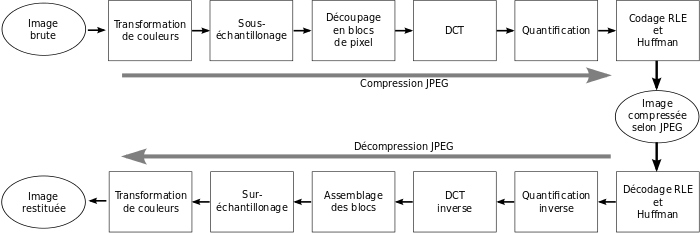
\includegraphics[width=120mm]{images/jpeg.png}
    \caption{Étapes de compression et décompression, issues de \autocite{jpeg}.}
    \label{fig:jpeg}
  \end{center}
\end{figure}

La figure \ref{fig:jpeg} liste toutes les étapes permettant de passer d'une image non compressée à une image compressée ainsi que le processus inverse. Les étapes sont sommairement : 

\begin{itemize}
  \item L'image est convertie dans l'espace YUV,
  \item Les canaux U et V sont sous-échantillonés,
  \item Chaque canal est découpé en blocs de 8$\times$8 pixels,
  \item Une DCT est appliquée à chacun de ces blocs pour avoir une matrice de $8\times 8$ coefficients,
  \item Chaque coefficient est quantifié selon une table de quantification (voir figure \ref{fig:quantization_table}) correspondant au facteur de qualité Q $\in$ \textit{\{1,2,3,...,100\}} et arrondi à l'entier le plus proche,
  \item Le tout est ensuite compressé à l'aide d'un codage entropique
\end{itemize}

C'est surtout l'étape de quantification qui va réduire la quantité d'information, et donc permettre de réduire la taille du fichier. Cette quantification, si elle est trop agressive va faire apparaître des artefacts de bloc, des blocs 8$\times$8 visibles (voir figure \ref{fig:blocs_artefacts}). C'est ce qui caractérise le JPEG, et qui permet de détecter un certain nombres de choses, comme l'altération d'images \autocite{bianchi2012image}, les doubles compressions \autocite{bianchi2012detection} ou encore dans notre cas les relations de parenté.

\begin{figure}[H]
  \begin{center}
    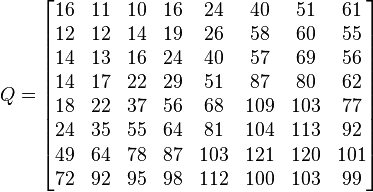
\includegraphics[width=60mm]{images/quantization_table.png}
    \caption{Exemple de table de quantification, issu de \autocite{jpeg}.}
    \label{fig:quantization_table}
  \end{center}
\end{figure}

\begin{figure}[H]
  \begin{center}
    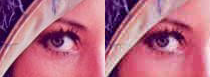
\includegraphics[width=120mm]{images/eyes.png}
    \caption{Artefacts de blocs, à gauche avec Q=90, à droite avec Q=20}
    \label{fig:blocs_artefacts}
  \end{center}
\end{figure}


\subsection{Estimation de la matrice de compression primaire dans les images JPEG doublement compressées}
\label{estimation_matrice_compression}

% \subsection{Estimation of primary quantization matrix in double compressed JPEG images}

% \subsection{Détection des recompressions JPEG}
% \citeauthornsc{feng2010jpeg} \autocite{feng2010jpeg}
\citeauthornsc{lukavs2003estimation} \autocite{lukavs2003estimation} proposent dans leur approche non seulement de détecter si une image est doublement compressée, mais également d'estimer les paramètres de la première compression. Pour bien comprendre la suite de leurs travaux, il convient d'expliquer plus en détail l'étape de quantification de JPEG.

La quantification se fait de la manière suivante :
\begin{equation}
  F^*(u,v) = \left \lfloor \frac{F(u,v) + \left \lfloor \frac{Q(u,v)}{2} \right \rfloor }{Q(u,v)} \right \rfloor,
  \label{eqn:quantization}
\end{equation}

où $F^*(u,v)$ est la valeur quantifiée, $F(u,v)$ est la valeur aux indices $u$ et $v$ dans la matrice 8$\times$8 de coefficients DCT et Q(u,v) et la valeur dans la table de quantification (figure \ref{fig:quantization_table}) à ces même indices.

Le calcul inverse est :
\begin{equation}
  F'(u,v) = F^*(u,v) * Q(u,v).
  \label{eqn:iquantization}
\end{equation}

où $F'(u,v)$ est la valeur issue de la quantification inverse aux indices $u$ et $v$ dans la matrice 8$\times$8 de coefficients DCT, $F^*(u,v)$ est la valeur quantifiée et Q(u,v) est la valeur dans la table de quantification (figure \ref{fig:quantization_table}) à ces même indices.

Nous voyons bien à partir des équations \ref{eqn:quantization} et \ref{eqn:iquantization} que le résultat après décompression sera un multiple de $Q(u,v)$ et que toutes les valeurs n'étant pas des multiples seront absentes.

La double compression est le fait de compresser deux fois une image, et donc de lui faire subir deux fois toutes les étapes de compression et de décompression, avec tous les arrondis et troncage que cela peut comporter. On notera, pour la double compression, $Q_{1}$ comme la matrice primaire, c'est à dire la table de quantification ayant servi à faire la première compression (inconnue donc), et $Q_{2}$ comme la matrice secondaire, ou la table de quantification actuelle, disponible dans l'en-tête du fichier JPEG. Les auteurs limitent la double compression aux cas où $Q_{1} \neq Q_{2}$.

Lors de la première compression, les coefficients sont quantifiés avec $Q_{1}$, ce qui veut dire que les coefficients sont des multiples de $Q_{1}$. Cependant, lorsque l'image est repassée du domaine fréquentiel au domaine spatial grâce à la DCT inverse, un certain nombre d'arrondis et de troncages se produisent pour rester dans l'intervalle [0..255]. Lors de la seconde compression, les coefficients DCT sont calculés à partir des ces valeurs inexactes, et donc ne seront pas multiples de $Q_{1}$, mais se concentreront autour. Ces nouveaux coefficients DCT seront ensuite quantifiés pour former la nouvelle image, doublement compressée.

Les auteurs ayant laissé de coté le cas où $Q_{1} = Q_{2}$, nous sommes en présence de deux cas : $Q_{1} > Q_{2}$ et $Q_{1} < Q_{2}$. Chacun des cas a des artefacts distincts et reconnaissables. La figure \ref{fig:histo} illustre un exemple de distributions ayant subi des quantifications, la figure \ref{ha} n'a subi qu'une seule quantification, la figure \ref{hb} correspond au cas où $Q_{1} > Q_{2}$ et la figure \ref{hc} correspond au deuxième cas. Un autre cas est délaissé, c'est celui où $Q_{1}$ est facteur $Q_{2}$, ce qui est assez logique, ils auront les même multiples, et il sera donc impossible de détecter quoi que ce soit, du moins en utilisant la méthode proposée ici.

L'estimation de la première table de quantification se limite aux basses fréquences, les hautes fréquences étant plus fortement quantifiées (souvent jusqu'à 0), elles contiennent moins d'informations et donc rendent leur estimation difficile.

Leur technique consiste à se munir d'une série de candidats pour la matrice primaire, notés $\{Q_{1,1},...,Q_{1,n}\}$. Ces tables de quantification viennent des tables utilisées dans les appareils photos, les téléphones portables ou les différentes implémentations de la compression JPEG. Parmi ces $\{Q_{1,1},...,Q_{1,n}\}$, le meilleur candidat, et donc la table la plus probable sera la table de quantification pour laquelle la différence entre l'histogramme de l'image et l'histogramme de l'image compressée avec $Q_{1,k}$ sera la plus faible.

L'identification de la matrice primaire peut être utile pour l'identification d'une relation parent-enfant entre deux images. Une image est potentiellement le parent d'une autre si sa table de quantification est la même que la matrice primaire d'une image recompressée avec une matrice secondaire. Cette méthode, bien que fort intéressante dans le cas de la phylogénie, perd en efficacité au-delà de la première recompression, et l'identification des différentes matrices peut devenir difficile à cause du bruit engendré par les multiples recompressions. 
 % où une image recompressée avec une matrice secondaire ayant la même matrice primaire qu'
% Cette technique est % parfaitement applicable dans le cas de l'identification de parent-en
\begin{figure}
  \begin{subfigure}{.33\textwidth}
    \centering
    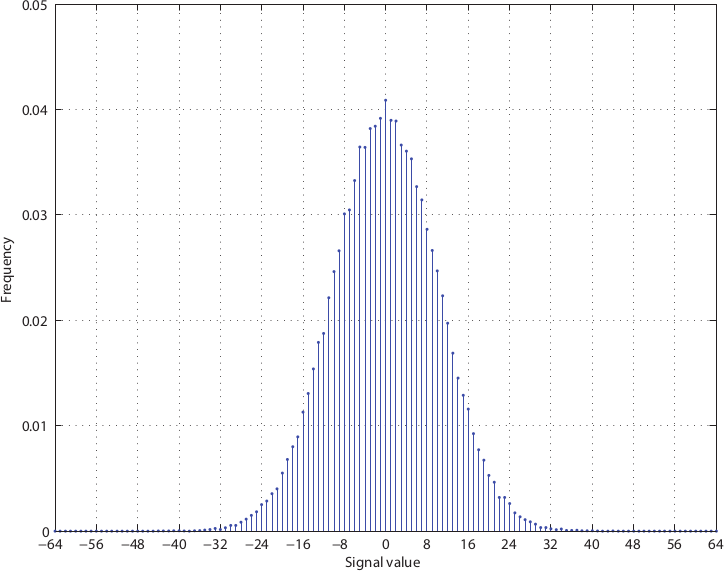
\includegraphics[width=\linewidth]{images/h1}
    \caption{quantifié une fois}
    \label{ha}
  \end{subfigure}
  \begin{subfigure}{.33\textwidth}
    \centering
    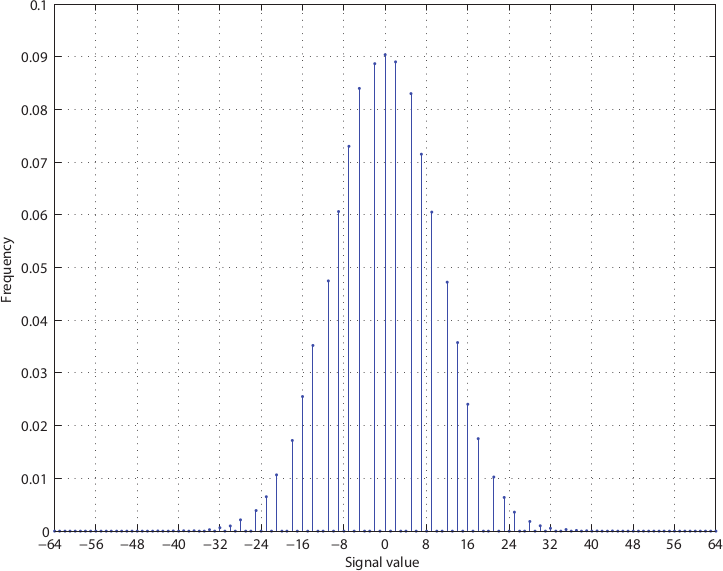
\includegraphics[width=\linewidth]{images/h2}
    \caption{re-quantifié, $Q_{1} > Q_{2}$}
    \label{hb}
  \end{subfigure}
  \begin{subfigure}{.33\textwidth}
    \centering
    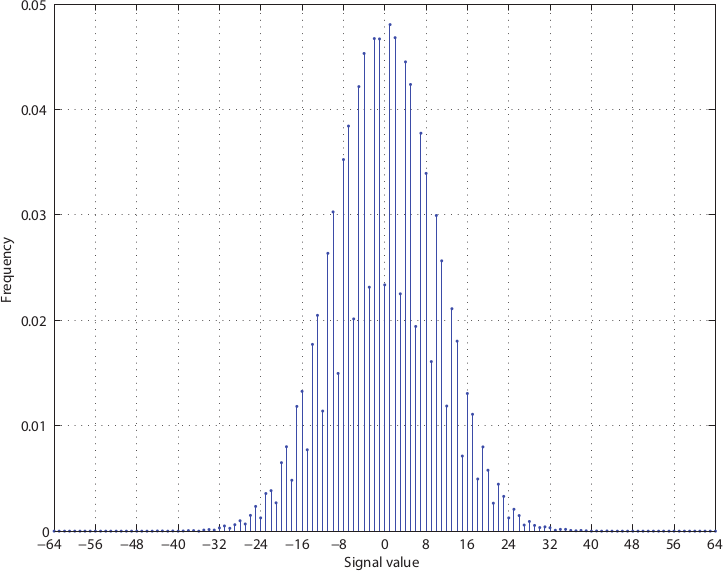
\includegraphics[width=\linewidth]{images/h3}
    \caption{re-quantifié, $Q_{1} < Q_{2}$}
    \label{hc}
  \end{subfigure}
  \caption{Exemple de quantifications sur l'histogramme d'une distribution normale avec des classes de largeur 1, issu de \autocite{feng2010jpeg}.}
  \label{fig:histo}
\end{figure}

\subsection{Détection des doubles compressions JPEG avec la même matrice de quantification}
% [en travaux]
% \autocite{huang2010detecting}
Comme expliqué section \ref{ipt}, nous tentons dans un premier temps d'identifier la génération $n$ d'une image $I_{n}$. Une tâche qui peut s'avérer difficile si les transformations sont minimes. En sachant que deux images $I_{m}$ et $I_{n}$ sont extrêmement similaires, sommes-nous en présence d'une double compression avec la même matrice de quantification, où l'une est le parent de l'autre, ou sommes-nous dans le cas où les images sont soeurs, et générées à partir d'une table de quantification identique ?

L'article de \citeauthornsc{huang2010detecting} \autocite{huang2010detecting} traite précisément de ce problème. Les auteurs constatent que les différences entre deux images issues de compressions successives diminuent lorsque le nombre de compressions augmente (voir figure \ref{d_courbe}), ce qui est en accord avec l'article de \citeauthornsc{lai2013block} \autocite{lai2013block}. Leur méthode, même si elle permet de détecter jusqu'à trois ou quatre compressions, est la plus efficace lorsque qu'il n'y a eu qu'une seule recompression.

\begin{figure}
  \begin{center}
    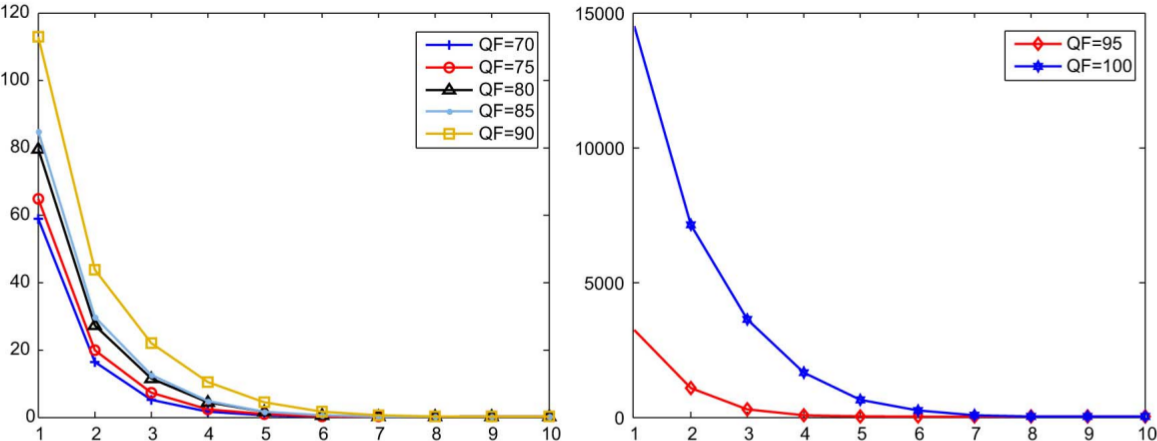
\includegraphics[width=130mm]{images/d_courbe}
    \caption{Diminution du nombre de valeurs différentes au fil des recompressions, issu de \autocite{huang2010detecting}.}
    \label{d_courbe}
  \end{center}
\end{figure}

Les auteurs vont s'appuyer sur trois signes distinctifs laissés par la compression JPEG : les erreurs de quantification, les erreurs de troncage et les erreurs d'arrondis. Leur méthode de détection est basée sur la perturbation aléatoire des coefficients DCT de l'image.

À partir d'une image $I$ compressée un nombre inconnu de fois, ils vont calculer $D$ comme le nombre de coefficients DCT différents entre $I$ et $I$ recompressée avec sa table de quantification, cette nouvelle image est notée $I'$

Ils vont ensuite perturber (ajouter ou soustraire 1) aléatoirement un nombre $n/r$ de coefficients DCT de $I'$ où $n$ est le nombre de coefficients modifiés par coefficient différent de zéro et r est un ratio choisi de manière experimentale.
% . Le nombre $n$ est déterminé à partir d'un ratio $r$ qu'il faudra choisir avec soin. Ce ratio est le nombre de coefficients modifiés par coefficient différent de zéro.

Cette image perturbée $I'$ est ensuite recompressée avec sa table de quantification pour donner $I''$. Le nombre $Dm$ est calculé comme le nombre de coefficients DCT différents entre $I'$ et $I''$. Cette étape est répétée $k$ fois, à chaque fois avec la nouvelle image obtenue. On obtient alors $\bar{D}m$, la moyenne de tous les $Dm$.

Une image I est doublement compressée si $\bar{D}m \geqslant D$. En effet, si c'est la première recompression, $D$ est grand (voir figure \ref{d_courbe}). C'est là qu'intervient le choix du ratio $r$. 

Ce ratio est calculé de manière experimentale, c'est à dire que grâce à une vérité terrain, et pour un certain ensemble d'images, les auteurs ont extrait le ratio donnant le meilleur résultat. Un des inconvénient de ce ratio est qu'il peut être sous-optimal pour un autre ensemble d'images, qui aura des caractéristiques différentes.

Un ratio mal choisi perturbera trop l'image et la modifiera plus que sa première recompression ou alors ne la perturbera pas suffisamment et l'image serait alors détectée à tort comme simplement compressée.

Cette méthode offre un moyen de détecter la présence de double compressions avec la même matrice de quantification, un cas probable dans le cadre des réseaux sociaux. Même si elle a été pensée pour la détection dans le cas de la première compression, cette méthode pourrait être étendue à la détection de la la $n^{ieme}$ et la $n+1^{ieme}$ compression. Contrairement aux auteurs, qui travaillent sur une image dans le vide, nous travaillons sur un ensemble d'images, et avons donc plus d'informations à notre disposition.
% nous ne travaillons pas sur une seule image, qui est la totalité de l'information disponible aux auteurs, nous travaillons sur un ensemble d'image. Nous disposons donc de bien plus d'informations, en plus des informations contenues dans les images, nous pouvons calculer des informations sur les images les unes par rapport aux autres. On pourrait donc très bien adapter cette méthode à la $n^{ieme}$ et la $n+1^{ieme}$ compression de deux images.

\subsection{Convergence des blocs lors de compressions successives}
\label{convergence}
L'intérêt de la méthode proposée par \citeauthornsc{CarneinSB2016TelltaleWatermarks} \autocite{CarneinSB2016TelltaleWatermarks} est l'estimation du nombre de compressions JPEG qu'a pu subir l'image, une estimation qui va au-delà de deux ou trois compression successives \autocite{huang2010detecting}\autocite{lukavs2003estimation}, il est en effet possible d'aller jusqu'à plusieurs centaines de compressions. Cette approche se base sur la notion de blocs cycliques.

Lors de compressions successives, une phénomène appelé \textit{convergence de bloc} peut être observé. Un bloc converge lorsque la valeur des pixels du bloc à la compression $t$ est égale à la valeurs des pixels à la compression $t + 1$, ce bloc est alors appelé stable \autocite{lai2013block}. Certains blocs cependant échappent à cet effet et exhibe un phénomène de cycle. C'est à dire que la valeur des pixels à la compression $t$ est égale à la valeur des pixels à la compression $t + n, n > 1$. Le deuxième type de bloc à échapper à ce phénomène est les blocs plats, ayant tous les pixels de la même valeur, ils ne peuvent pas être cycliques puisque tous les coefficients DCT sauf le premier sont nuls.

Ces blocs sont nommés blocs compteurs. Ainsi, si un bloc de l'image a un cycle de longueur $l=9$, il sera possible de savoir, modulo $l$, combien de compressions a subi l'image. Et avec plus de blocs, ayant chacun des $l$ différents, il est possible d'aller bien plus loin dans le nombre de compressions. Prenons l'exemple de trois blocs pour lesquels $l_{1} = 2$, $l_{2} = 5$ et $l_{3} = 9$. Le nombre maximum de compressions successives qu'il sera possible d'estimer est le \textit{plus petit commun multiple} des ces longueurs, autrement dit, $ppcm(2, 5, 9) = 90$, soit 90 compressions successives, et pour l'exemple illustré par la figure \ref{fig:insertion_blocs}, $ppcm(6, 7, 10, 12) = 420$.

\paragraph{}
Les auteurs proposent deux approches pour les blocs cycliques. La première consiste à détecter les blocs cycliques à l'aide d'une recherche exhaustive sur l'ensemble des blocs et un certain nombre de compressions puis sélectionner les blocs intéressants. Cette méthode, bien qu'étant la plus simple, et ne modifiant pas l'image, peut cependant rencontrer des problèmes lorsqu'elle comporte un grand nombre de blocs plats, il peut en effet être difficile de trouver des blocs ayant des cycles de longueur intéressante. La deuxième approche proposée est donc d'insérer des blocs artificiellement créés dans l'image (voir figure \ref{fig:insertion_blocs}). 

Cette méthode nécessite de prendre un certain nombre de précautions et requiert une protection (padding) autour des blocs insérés. L'algorithme de sur-échantillonage est en effet parfois amené à utiliser les valeurs des pixels des blocs adjacents pour un meilleur rendu et provoquer un effet de débordement (spill over) des valeurs \autocite{carnein2015forensics}, ce qui modifie le bloc artificiellement créé (dans le vide) et donc modifie son cycle, rendant nulle son information.

\begin{figure}[H]
  \begin{center}
    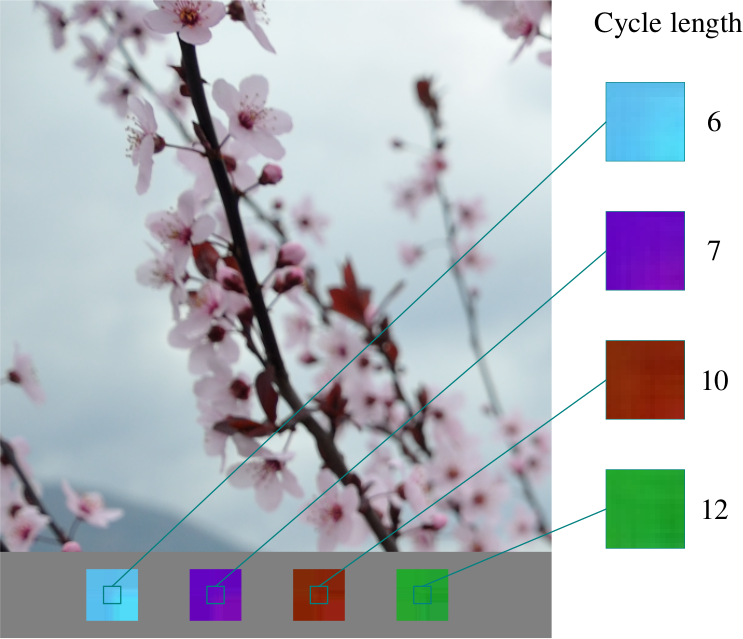
\includegraphics[width=80mm]{images/insertion_blocs}
    \caption{Exemple d'insertion de blocs, issu de \autocite{CarneinSB2016TelltaleWatermarks}.}
    \label{fig:insertion_blocs}
  \end{center}
\end{figure}


%%%%parler du calcul des blocs et tout
\paragraph{}

Si l'insertion de blocs artificiels dans l'image est mise de coté, technique qui ne serait pas possible dans notre cas, le principal inconvénient de cette méthode 
 est qu'elle se restreint à des images ayant toutes le même facteur de qualité, et en particulier $Q = 100$, pour lequel les cycles sont les plus longs, et donc donnent le plus d'informations. C'est un cas spécifique pour notre cadre d'utilisation : les réseaux sociaux, où les facteurs de qualité de compression varient en fonction de l'application utilisée. Cette méthode est en effet plus orientée vers le tatouage et le traçage d'images.

\section{Distances entre distributions}
% [en travaux]
% \autocite{oikawa2015distances}

Dans l'approche que nous proposons de développer lors de ce stage, il nous sera nécessaire de calculer des distances entre des distributions. C'est la raison pour laquelle nous avons décidé passer en revue un certain nombre de distance dans l'état de l'art.

Commençons par définir la différence entre une distance et une divergence. Une distance, contrairement à une divergence, est symétrique, c'est à dire que $distance(I_{m},I_{n}) = distance(I_{n},I_{m})$, et elle vérifie l'inégalité triangulaire. Une distance est parfaite pour mesurer la proximité entre deux objets. Elle est cependant dans l'incapacité de nous donner des indications sur une direction.

\paragraph{}

Nous travaillons avec une relation asymétrique (relation parent-enfant), une divergence semble donc être mieux adaptée pour estimer la direction de cette relation (voir chapitre \ref{chap3}).

Il peut cependant être envisagé d'utiliser une distance pour estimer une direction si le calcul de la distance est fait après avoir appliqué une opération asymétrique. Comme expliqué chapitre \ref{chap2} section \ref{etude}, \citeauthornsc{dias2012image} mappent une image dans le domaine d'une autre, ce qui est une opération asymétrique, et donc qui permettrait d'utiliser une distance. C'est pourquoi nous traiterons aussi bien les distances que les divergences.

\paragraph{}

 Il existe un grand nombre de mesure de distances \autocite{cha2007comprehensive}, aussi, nous ne parlerons que des distances entre distributions les plus utilisées. Nous n'entrerons cependant pas dans les détails théoriques de ces calculs de distance, qui nécessiteraient une étude bibliographique à eux seuls, nous utiliserons ces distances comme des boites noires et choisirons de manière expérimentale la plus adaptée. Nous allons donc donner pour chaque distance son nom et sa formule.

Dans la suite de cette section, $P$ et $Q$ seront des densités de probabilité.

\subsection{Les distances}

La distance euclidienne : 
\begin{equation}
  D_{euc}(P,Q) = \sqrt{\sum\limits_{i=1}^{d}|P_{i} - Q_{i}|^2}
\end{equation}
\\
La distance de Bhattacharyya :

\begin{equation}
  D_{B}(P,Q) = -ln\sum\limits_{i=1}^{d} \sqrt{P_{i}Q_{i}}
\end{equation}
\\
L'index de Jaccard est donné comme : 

\begin{equation}
  S_{Jac}(P,Q) = \frac{\sum\limits_{i=1}^{d} P_{i}Q_{i}}{\sum\limits_{i=1}^{d} P^{2}_{i} + \sum\limits_{i=1}^{d} Q_{i}^{2} - \sum\limits_{i=1}^{d} P_{i}Q_{i}}
\end{equation}

Il correspond à la taille de l'intersection entre deux distributions divisé par la taille de leur union. La distance de Jaccard est :

\begin{equation}
  D_{Jac}(P,Q) = 1 - S_{Jac}(P,Q) = \frac{\sum\limits_{i=1}^{d} (P_{i} - Q_{i})^2}{\sum\limits_{i=1}^{d} P^{2}_{i} + \sum\limits_{i=1}^{d} Q^{2}_{i} - \sum\limits_{i=1}^{d} P_{i}Q_{i}}
\end{equation}

\subsection{Les divergences}

La divergence de Kullback–Leibler :%\autocite{kullback1951} :

\begin{equation}
  D_{KL}(P||Q) = \sum\limits_{i=1}^{d} P_{i}\ log\ \frac{P_{i}}{Q_{i}}
\end{equation}
\\
La K divergence : 
\begin{equation}
  D_{kdiv}(P||Q) = \sum\limits_{i=1}^{d} P_{i}\ log\ \frac{2P_{i}}{P_{i}+Q_{i}}
\end{equation}

\vspace{8mm}
Au travers de cet état de l'art, nous avons pu voir différentes méthodes de calcul de l'arbre phylogénétique et avons vu que la difficulté se trouve dans l'estimation des relations de parenté entre les images. Ce que nous avons tenté de résoudre en nous intéressant à l'analyse des compressions multiples, analyse qui est loin d'être triviale et qui souvent se limite aux premières recompressions. Nous avons également vu plusieurs calculs de distances qui serviront eux aussi à estimer les relations de parenté entre images.

% \chapter{Notre approche}
% Ce chapitre est consacré à présenter notre approche, nous y détaillons notre approche, formalisée par un théorème, puis nous présentons un algorithme permettant de reconstruire l'arbre de phylogénie.
% \label{chap:notre_approche}
% \section{Principe et théorème}
% Pour tout couple d'images de notre ensemble, nous allons tenter de nier qu'il existe une relation de parenté, cela va permettre d'extraire une matrice binaire, appelée \textit{matrice de parenté}, de la taille de l'ensemble d'images, où une valeur à 1 indiquera une relation de parenté et une valeur à 0 en indiquera l'absence. À noter une fois de plus que ce n'est pas forcément un parent direct mais plutôt un ancêtre. \\ \indent
% Nous pouvons noter plusieurs choses intéressantes de l'exemple illustré figure \ref{parentage_tree}. Toutes les valeurs de la colonne de l'image $I_{2}$ sont à 1 , c'est à dire que c'est un parent commun à toutes les autres images, et sa ligne n'a que des 0, elle n'a donc aucun parent. Nous nous servons de ce principe pour la reconstruction de l'arbre à partir de la matrice : une image qui n'a pas de parent est la racine. Nous pouvons également remarquer les colonnes où toutes les cases sont à 0, cela veut dire que ces images ne sont les parents de personne, et donc sont des feuilles.

% Nous avons formalisé ce principe en un théorème présenté ci-dessous: 
% \newtheorem*{marqueur}{Définition}
% \begin{marqueur}
%   Un \textbf{marqueur} est une caractéristique locale ou globale extraite de l'image qui indique qu'une certaine opération a été effectuée. Ce marqueur va se transmettre aux enfants de l'image, et serviront potentiellement à prouver qu'une image n'est pas le parent d'une autre.

% Par exemple une image en noir et blanc ne peut pas être le parent d'une image couleur car le marqueur ``couleur'' est absent de l'image en noir et blanc.
% \end{marqueur}

% \newtheorem*{fonction}{Définition}
% \begin{fonction}
%   Soit $f(I_{m},I_{n})$ une fonction qui pour tout couple d'images $(I_{m}, I_{n})$ détecte à chaque fois qu'il est présent un marqueur indiquant qu'il n'y a pas de relation de parenté entre $I_{m}$ et $I_{n}$. Cette fonction est appelée fonction de négation. Notons que ce type de fonction est plus ou moins abstrait et qu'un des objectifs du stage sera d'essayer d'en proposer au moins une.
%  % est nous devrons la trouver dans la suite du stage.
% \end{fonction}

% \newtheorem*{parentage}{Théorème}
% \begin{parentage}
%   % Supposons qu'il existe une fonction $f(.,.)$ qui pour tout couple d'image passé en paramètre détecte à chaque fois qu'il est présent un marqueur prouvant qu'il n'y a pas de relation de parenté entre ces deux images.
%   Pour tout couple d'images ($I_{m}$, $I_{n}$) d'un ensemble de near-duplicates, s'il n'existe pas de marqueur prouvant que $I_{m}$ n'est pas le parent de $I_{n}$, alors il y a une relation parent-enfant entre $I_{m}$ et $I_{n}$, $I_{m}$ $\to$ $I_{n}$.
% \end{parentage}

% \begin{proof}
%   Si $f(I_{m},I_{n})$ ne parvient pas à trouver de marqueur prouvant que $I_{m}$ n'est pas de parent de $I_{n}$ alors c'est que ce marqueur n'existe pas et donc que $I_{m}$ est le parent de $I_{n}$, avec $m < n$.
% \end{proof}

\chapter{Méthode de calcul de phylogénie à l'aide des caractéristiques des coefficients DCT d'une bitmap}
\label{chap3}

Nous tentons de reconstruire l'arbre de phylogénie d'un ensemble de near-duplicates. Contrairement aux approches de l'état de l'art qui utilisent des algorithmes de construction d'arbre complexes pour reconstruire l'arbre à partir d'une dissimilarity matrix, nous allons prendre une décision binaire entre deux image, à savoir ``Cette image est-elle le parent de cette autre image ?''. Cela nous permet de nous concentrer sur les images et leurs caractéristiques et avoir un algorithme de construction d'arbre simple. La figure \ref{fig:method_schema} présente notre méthode. Dans ce chapitre, nous commencerons pas présenter les principes et théorème sur lesquels s'appuient notre méthode section \ref{sec:method} puis nous détaillerons directement le calcul de la période de chaque coefficient DCT section \ref{sec:extraction} sans expliquer comment ils ont été obtenus, c'est en effet largement traité dans \autocite{wallace1992jpeg}, nous expliquerons comment est estimé le facteur de qualité en \ref{sec:estimation} pour ensuite détailler l'estimation du parent et la construction de l'arbre sections \ref{sec:parent} et \ref{sec:reconstruction} et nous terminerons par le filtrage des doublons section \ref{sec:filtrage}.

\begin{figure}[H]
  \begin{center}
    % \begin{tikzpicture}[auto, distance=2in,sibling distance=.25in]
    \scalebox{0.85}{
      \begin{tikzpicture}[auto,node distance=2.8cm]

        \tikzstyle{every state}=[shape=rectangle,minimum width=1.3in,text width=1.3in, align=center,fill=blue!30]
        % \tikzstyle{every data}=[shape=circle,minimum width=1.3in,text width=1.3in, align=center,fill=blue!30]

        \node[draw=none,fill=none,minimum width=1.1in,text width=1.1in, align=center] (A) {Ensemble de near-duplicates};
        \node[state] (B) [right=0.7cm of A] {DCT sur chaque image};

        \node[draw=none,fill=none,minimum width=1.1in,text width=1.1in, align=center, right=0.7cm of B] (C) {Coeffs DCT de chaque image};
        \node[state] (D) [right=0.7cm of C] {Extraction de la période de chaque coefficient DCT};

        \node[draw=none,fill=none,minimum width=1.1in,text width=1.1in, align=center, right=0.7cm of D] (E) {Tables de quantification estimées};
        \node[state] (F) [below=0.7cm of E] {Estimation du facteur de qualité};

        \node[draw=none,fill=none,minimum width=1.1in,text width=1.1in, align=center, left=0.7cm of F] (G) {$Q_f$ de chaque image};
        \node[draw=none,fill=none,minimum width=1.1in,text width=1.1in, align=center, below=0.3cm of G] (H) {Images};
        \node[state] (I) [left=0.7cm of G] {Estimation du parent};

        \node[draw=none,fill=none,minimum width=1.1in,text width=1.1in, align=center, left=0.7cm of I] (J) {Matrice de parenté};
        \node[state] (K) [left=0.7cm of J] {Construction de l'arbre};

        \node[draw=none,fill=none,minimum width=1.1in,text width=1.1in, align=center, below=1.2cm of K] (L) {Arbre non traité};
        \node[state] (M) [right=0.7cm of L] {Filtrage des doublons};
        
        \node[draw=none,fill=none,minimum width=1.1in,text width=1.1in, align=center, right=0.7 of M] (N) {Arbre de phylogénie};

        \path [->] (A) edge node[left] {} (B);
        \path [->] (B) edge node[left] {} (C);      
        \path [->] (C) edge node[left] {} (D);      
        \path [->] (D) edge node[] {} (E);      
        \path [->] (E) edge node[right] {} (F);      
        \path [->] (F) edge node[right] {} (G);      
        \path [->] (G) edge node[left] {} (I); 
        \path [->] (H) edge node[left] {} (I);
        \path [->] (I) edge node[left] {} (J);
        \path [->] (J) edge node[left] {} (K);
        \path [->] (K) edge node[left] {} (L);
        \path [->] (L) edge node[left] {} (M);
        \path [->] (M) edge node[left] {} (N);
      \end{tikzpicture}}
    \caption{Schéma de notre méthode}
    \label{fig:method_schema}
  \end{center}
\end{figure}

\section{Principe et théorème}
\label{sec:method}
Pour tout couple d'images de notre ensemble, nous tentons donc de prendre une décision binaire, qui vas nous permettre d'extraire une \textit{matrice de parenté}. Rappelons la que nous tentons de savoir si une image est l'ancêtre d'une autre, et pas seulement son parent direct. Nous mettons en place un framework pour tenter de résoudre ce problème : 
% nous allons tenter de nier qu'il existe une relation de parenté, cela va permettre d'extraire une matrice binaire, appelée \textit{matrice de parenté}, de la taille de l'ensemble d'images, où une valeur à 1 indiquera une relation de parenté et une valeur à 0 en indiquera l'absence. À noter une fois de plus que ce n'est pas forcément un parent direct mais plutôt un ancêtre. \\ \indent

\newtheorem*{marqueur}{Définition}
\begin{marqueur}
  Un \textbf{marqueur} est une caractéristique locale ou globale extraite de l'image qui indique qu'une certaine opération a été effectuée. Ce marqueur va se transmettre aux enfants de l'image, et serviront potentiellement à prouver qu'une image n'est pas le parent d'une autre.

Par exemple une image en noir et blanc ne peut pas être le parent d'une image couleur car le marqueur ``couleur'' est absent de l'image en noir et blanc.
\end{marqueur}

\newtheorem*{fonction}{Définition}
\begin{fonction}
  Soit $f(I_{m},I_{n})$ une fonction qui pour tout couple d'images $(I_{m}, I_{n})$ détecte à chaque fois qu'il est présent un marqueur indiquant qu'il n'y a pas de relation de parenté entre $I_{m}$ et $I_{n}$. Cette fonction est appelée fonction de négation. Notons que ce type de fonction est plus ou moins abstrait et que c'est ici que se situe la difficulté.
\end{fonction}

\newtheorem*{parentage}{Théorème}
\begin{parentage}
  % Supposons qu'il existe une fonction $f(.,.)$ qui pour tout couple d'image passé en paramètre détecte à chaque fois qu'il est présent un marqueur prouvant qu'il n'y a pas de relation de parenté entre ces deux images.
  Pour tout couple d'images ($I_{m}$, $I_{n}$) d'un ensemble de near-duplicates, s'il n'existe pas de marqueur prouvant que $I_{m}$ n'est pas le parent de $I_{n}$, alors il y a une relation parent-enfant entre $I_{m}$ et $I_{n}$, $I_{m}$ $\to$ $I_{n}$.
\end{parentage}

\begin{proof}
  Si $f(I_{m},I_{n})$ ne parvient pas à trouver de marqueur prouvant que $I_{m}$ n'est pas de parent de $I_{n}$ alors c'est que ce marqueur n'existe pas et donc que $I_{m}$ est le parent de $I_{n}$, avec $m < n$.
\end{proof}

Ce framework a été imaginé lors de l'étude bibliographique, nous allons ensuite présenter notre méthode, et voir comment il a été utilisé et adapté.


\section{Estimation du facteur de qualité d'une image JPEG}
Nous travaillons sur des images ayant subi une compression JPEG. Ces images, au fil de leurs voyages sur les réseaux sociaux, on pu changer de format et avoir été convertie au format PNG par exemple. L'information du facteur de qualité utilisé pour compresser l'image, indispensable à nos calculs, a été perdue. Nous proposons donc d'estimer le facteur de qualité d'une bitmap n'ayant pas subi d'autre compression avec perte que le JPEG.

% \section{Estimation du pas de quantification}
\subsection{Estimation de la table de quantification}
\label{sec:extraction}
Nous avons besoin des coefficients DCT de l'image pour pouvoir estimer la table de quantification. Deux choix s'offrent à nous : calculer une DCT à partir d'une bitmap, ou compresser une bitmap au format JPEG avec $Q_f = 100$ et lire directement les coefficients DCT. Le deuxième choix s'avère être le plus simple à mettre en place et c'est celui que nous avons utilisé.

Comme expliqué section \ref{estimation_matrice_compression}, les valeurs des coefficients DCT vont se rassembler autour des multiples de $q$, qui est le nombre utilisé pour la quantification. Chaque coefficient DCT forme donc un signal périodique, de période $q$. C'est cette période que nous allons tenter d'estimer. L'autocorrélation est la technique traditionnellement utilisée pour extraire une période.

% \subsection{Calcul de la table de quantification}
Chaque implémentation de la compression JPEG possède sa propre table de quantification, un exemple de table de quantification est donnée figure \ref{fig:quantization_table}. La table de quantification $base(.,.)$ est donnée pour $Q_f = 50$, pour obtenir les tables de quantification pour les différents $Q_f$, les formules \ref{eqn:jpeg_1} et \ref{eqn:jpeg_2} sont utilisées. Cela permet, si c'est une table standard qui est utilisée, de ne pas avoir à stocker la table dans l'en-tête du fichier JPEG et de pouvoir la calculer à partir de $Q_f$.

\begin{equation}
  si\ Q_f < 50\ \ \ \ \ \  Q_s = 5000 / Q_f\ \ \ \ \  sinon\ \ \ \ \ Q_s = 200 - (Q_f \times 2)
  \label{eqn:jpeg_1}
\end{equation}

\begin{equation}
  q(u,v) = \frac{(base(u,v) \times Q_s) - 50}{100}\ \ \ \ \ en\ bornant\ q(u,v)\ par\ 1\ et\ 255
  \label{eqn:jpeg_2}
\end{equation}

\subsection{L'autocorrélation et la détection de pics}
L'autocorrélation est la multiplication du signal avec lui-même à différents points du temps. Ainsi, l'autocorrélation d'un signal périodique aura des valeurs maximales (des pics) lorsque le décalage temporel $\uptau$ est un multiple de la période, et donc que le signal est le plus similaire avec lui-même.

Nous savons que les valeurs du pas de quantification sont bornées par 1 et 255, nous allons donc calculer l'autocorrélation entre ces deux bornes. Un exemple de signal et son autocorrélation est disponible figures \ref{fig:signal} et \ref{fig:autocorrel}.

\begin{figure}
  \begin{subfigure}{.5\textwidth}
    \centering
    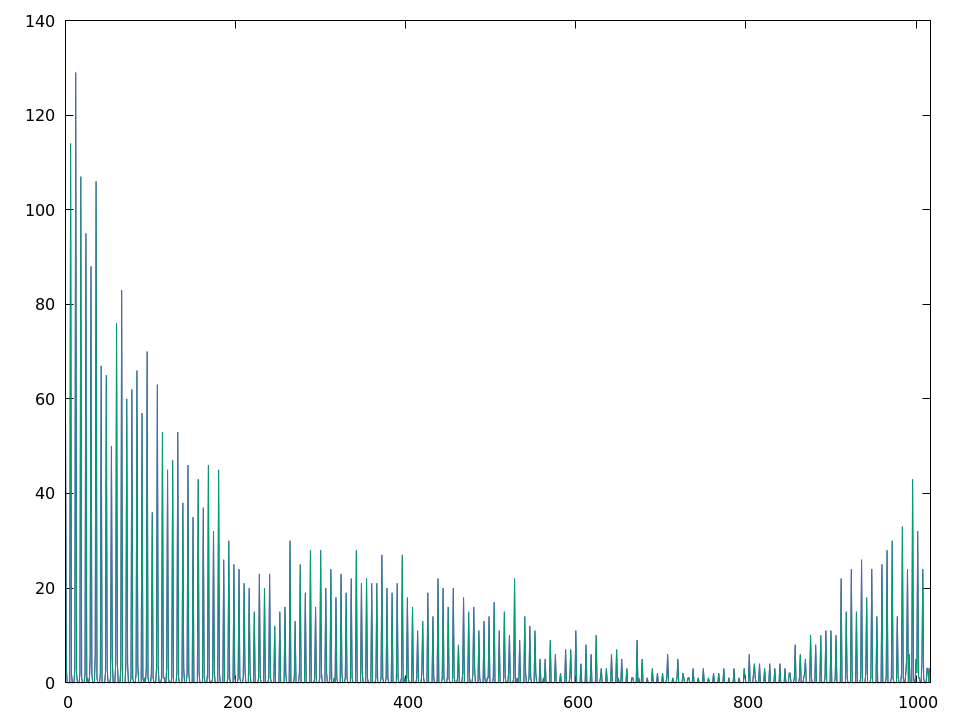
\includegraphics[width=\linewidth]{images/signal}
    \caption{Histogramme du coefficient DC d'une image}
    \label{fig:signal}
  \end{subfigure}
  \begin{subfigure}{.5\textwidth}
    \centering
    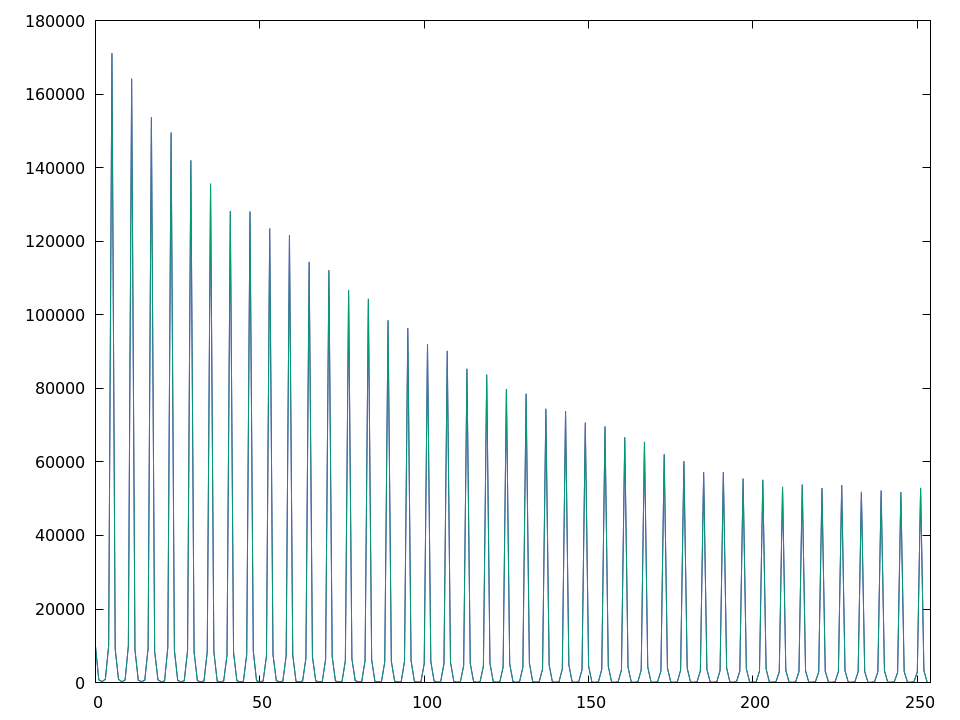
\includegraphics[width=\linewidth]{images/autocorrelation}
    \caption{Autocorrélation de ce signal}
    \label{fig:autocorrel}
  \end{subfigure}
  \caption{Exemple de signal et son autocorrélation}
\end{figure}

\begin{figure}
  \begin{subfigure}{.5\textwidth}
    \centering
    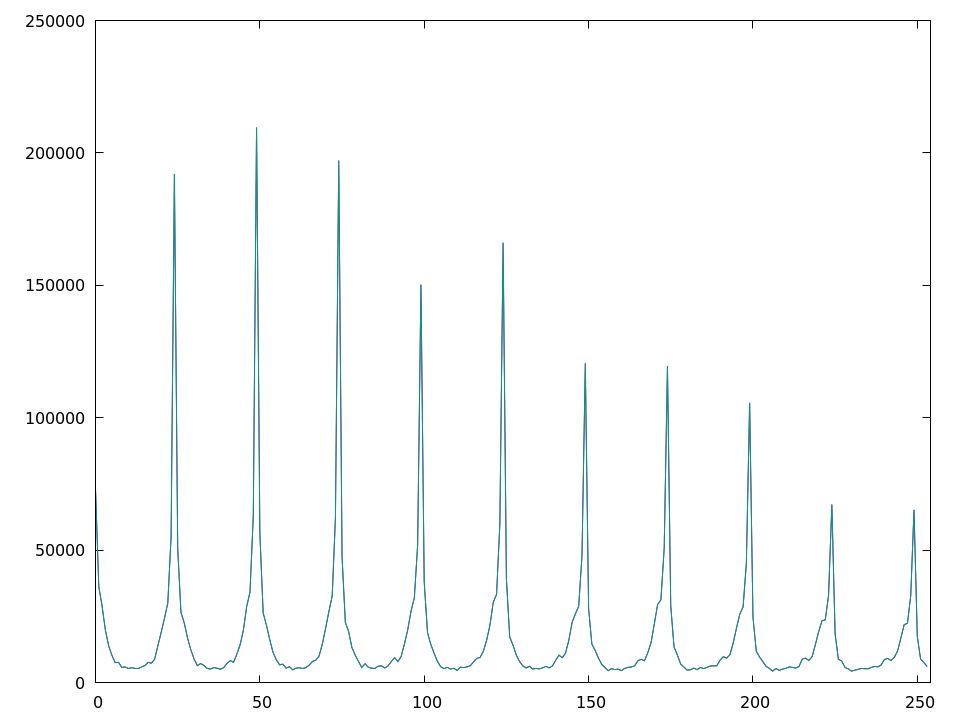
\includegraphics[width=\linewidth]{images/signal_noise}
    \caption{Exemple de bruit entre les pics}
  \end{subfigure}
  \begin{subfigure}{.5\textwidth}
    \centering
    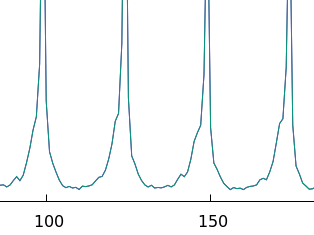
\includegraphics[width=\linewidth]{images/signal_noise_zoom}
    \caption{Zoom sur le bruit}
  \end{subfigure}
  \caption{Présence de bruit entre les pics}
  \label{fig:signal_noise}
\end{figure}

La période va ensuite être le delta entre deux pics consécutifs. La détection d'un pic est triviale lorsque le signal est propre et ne comporte aucun bruit, une valeur est un pic si la valeur précédente et la valeur suivante sont strictement inférieures. Nous ne sommes hélas pas dans le cas idéal, comme illustré figure \ref{fig:signal_noise}, où de faux pics peuvent être détectés si on prend le signal en l'état.

La méthode la plus simple, efficace,  peu coûteuse en temps de calcul et facile à mettre en place est de ne garder que les valeurs supérieures à un seuil. Notre seuil est calculé comme cinq fois la valeur moyenne de l'autocorrélation. Un exemple est disponible figure \ref{fig:signal_filtered}

\begin{figure}[H]
    \centering
    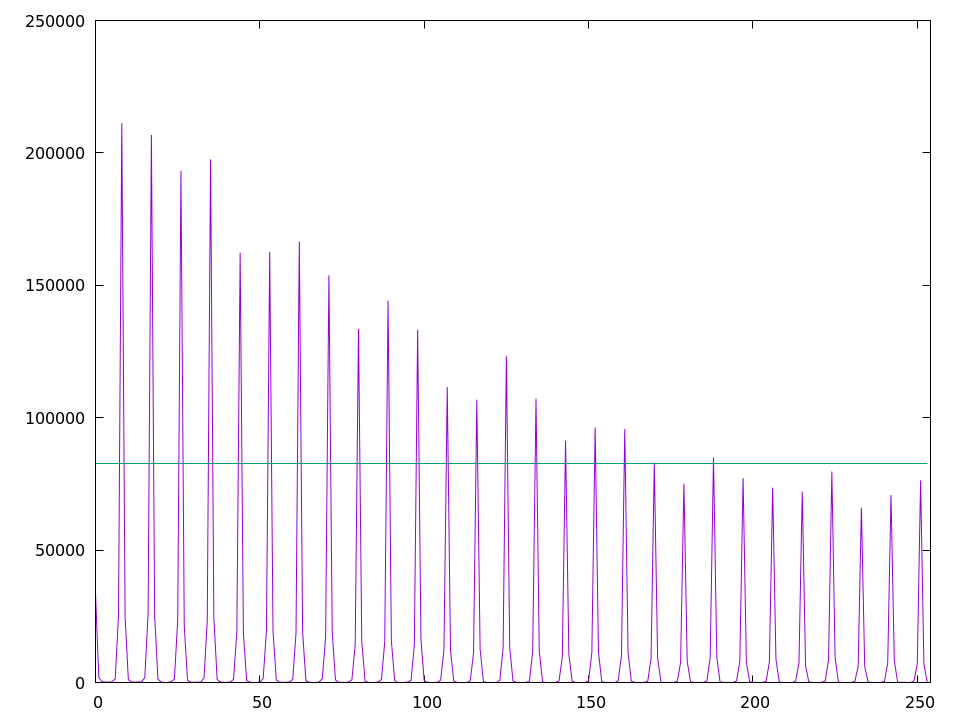
\includegraphics[width=0.5\linewidth]{images/autocorrelation_filtered}
    \caption{Exemple d'autocorrélation avec un seuil (en vert)}
    \label{fig:signal_filtered}
\end{figure}

Seuls les quelques premiers pics sont conservés, nous sommes en effet certains qu'ils seront au dessus du seuil, et donc qu'il n'y aura pas de pic manquant (comme les pics de la droite de la figure \ref{fig:signal_filtered} qui alternent entre au dessus et en dessous du seuil) qui viendrait fausser le calcul de la période.

Il est important de noter que cette technique donne de très bons résultats, mais seulement dans notre cas d'étude, c'est à dire que le $Q_f$ d'une image est strictement inférieur à celui de son parent. Dans le cas où le $Q_f$ peut être supérieur, comme expliqué section \ref{estimation_matrice_compression}, des doubles pics peuvent apparaître et rendre compliqué le calcul de la période. Un exemple est disponible figure \ref{fig:double_peaks}.

\begin{figure}[H]
    \centering
    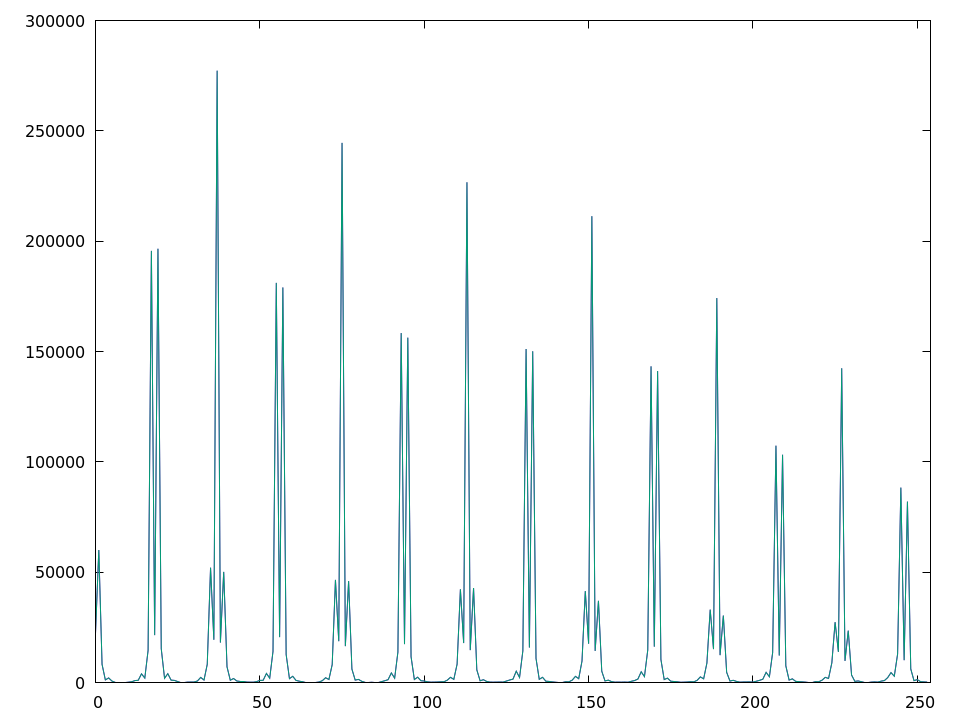
\includegraphics[width=0.5\linewidth]{images/autocorrelation_double}
    \caption{Exemple d'autocorrélation avec des doubles pics}
    \label{fig:double_peaks}
\end{figure}

Cette opération est donc répétée pour les 35 premiers coefficients DCT de l'image pour obtenir $\widehat{q}(u,v)$ la table de quantification estimée. Nous n'estimons que les 35 premiers coefficients DCT de l'image, la quantification des derniers coefficients est trop importante et il y a trop de valeurs à zéro, et donc pas assez d'informations pour estimer de manière précise la période.

\subsection{Calcul de $Q_f$ à partir de $\widehat{q}(u,v)$}
\label{sec:estimation}
Il va maintenant falloir calculer $Q_f$ à partir de $\widehat{q}(u,v)$, la table de quantification précédemment estimée. Deux choix s'offrent à nous : regarder parmi toutes les tables $q_n(u,v),\ n\in\{1..100\}$ laquelle est la plus similaire (avec un calcul de distance par exemple), ou utiliser les équations \ref{eqn:jpeg_1} et \ref{eqn:jpeg_2}. 

L'avantage de la première méthode est qu'elle nous donne directement $Q_f$, c'est la table pour laquelle la distance entre $q_n(u,v)$ et $\widehat{q}(u,v),\ n\in \{1..100\}$ est la plus faible. Le principal désavantage de cette technique est qu'elle est coûteuse en temps de calcul, en plus de manquer de précision.

L'autre méthode, même si elle ne demande presque aucun calcul, a un défaut majeur, elle ne permet pas d'obtenir $Q_f$. On peut en effet obtenir $Q_s$ à partir de l'équation \ref{eqn:jpeg_2}, mais il n'est pas possible d'obtenir $Q_f$ à partir de $Q_s$ sans savoir si $Q_f$ est supérieur à 50.

Nous avons choisi de conjuguer les deux méthodes. Nous obtenons une première estimaton de $Q_f$ en regardant parmi toutes les tables laquelle est la plus similaire à l'aide d'un calcul de distance, nous appelons cette étape l'estimation primaire. Avec cette estimation primaire de $Q_f$, nous affinons la précision du calcul en utilisant les équations \ref{eqn:jpeg_1} et \ref{eqn:jpeg_2}. Ainsi, un $Q_f*$ va être calculé pour chaque coefficient de la table de quantification $\widehat{q}(u,v)$, le $Q_f$ final est la moyenne de l'ensemble de tous les $Q_f*$. Cette étape est appelée estimation secondaire.
% Premièrement nous obtenons une estimation grossière de $Q_f$ en regardant parmi toutes les tables laquelle est la plus similaire, puis avec cette estimation de $Q_f$ nous calculons, manière plus précise le vrai $Q_f$ à l'aide des équations \ref{eqn:jpeg_1} et \ref{eqn:jpeg_2}. Le $Q_f$ final est donc la moyenne des $Q_f$ obtenus pour chaque coefficient DCT.

\section{Estimation du parent}
\label{sec:parent}
Le facteur de qualité utilisé pour compresser l'image nous est indispensable pour estimer le parent. En plus d'être un marqueur très efficace pour filtrer les images ne pouvant pas être le parent, le facteur de qualité nous sert à normaliser les images pour pouvoir les comparer.

Nous partons du principe que la compression JPEG est une opération déterministe, elle donnera, pour une même implémentation, toujours le même résultat. Cela implique que toutes les compressions d'une certaine image avec le même facteur de qualité seront strictement identiques, et ce quelque soit le nombre de compressions qu'à pu subir l'image au préalable.

Nous nous sommes limités aux compressions JPEG comme expliqué précédemment, nous savons donc que pour passer d'une image parent à son image enfant, l'image parent aura été recompressée. L'image parent est donc à une compression de l'image enfant.

Nous allons utiliser ces précédents principes pour identifier avec précision le parent : 
\paragraph{}

Soit $I_m$ et $I_n$ deux images et $Q_{f_{m}}$ et $Q_{f_{n}}$ leurs facteurs de qualité respectifs, et $C(I,Q)$ l'opérateur de compression, avec $I$ l'image et $Q$ le facteur de qualité.
\\
Si $I_m = C(I_n, Q_{f_{m}})$, alors $I_n$ est le parent direct de $I_m$.
\paragraph{}

C'est en pratique presque aussi simple qu'en théorie, on voit bien que tout dépend du facteur de qualité, or nous estimons ce facteur de qualité, et il peut arriver qu'il ne soit pas exact, mais un peu trop grand ou un peu trop petit. Nous n'allons donc pas nous contenter de comparer les images compressées avec le $Q_f$ estimé, nous allons également regarder les $Q_f$ alentours jusqu'à ce qu'un parent soit détecté. La précision de l'estimation du parent est donc directement corrélée avec le temps de calcul de notre algorithme. 

 % regarder les $Q_f$ alentours (de $Q_f - 2$ à $Q_f + 2$ par exemple). La précision de l'estimation du parent est donc directement corrélée avec l'exactitude de l'estimation du facteur de qualité.

\paragraph{}
Cette méthode, même si elle donne d'excellents résultats pour trouver le parent direct, ne permet pas de trouver les grands parents ou les ancêtres plus éloignés. Nous tentons en effet de prendre une décision binaire : ``Cette image est-elle le parent de cette autre image ?''. Une décision binaire est difficile lorsque l'on travaille sur des valeurs dont les bornes dépendent de l'input. Il est alors difficile d'utiliser des seuils pour correctement filtrer les valeurs. L'alternative logique est de ne pas utiliser de seuil, et comparer les valeurs entre elles. 

On peut raisonnablement penser que l'ancêtre le plus probable est l'image ayant la plus petite valeur (issue d'une métrique quelconque) parmi toutes les autres valeurs. Le problème est que l'on perd alors le principe de décision binaire entre deux images.

\section{Reconstruction de l'arbre}
\label{sec:reconstruction}
La phase d'estimation des parent nous a permis de créer une matrice binaire de taille $n\times n$, $n$ étant le nombre d'images dans le set. Cette matrice est appelée \textit{matrice de parenté}. Une valeur à 1 à l'indice $(i,\ j)$ de cette matrice indiquera que l'image $I_i$ est un des ancêtres de $I_j$. Une valeur à 0 indiquera l'absence de parenté. Un exemple d'arbre et de matrice de parenté est disponible figure \ref{parentage_tree}. On peut noter plusieurs choses intéressantes de cet exemple. Une colonne où toutes les valeurs sont à 0 indiquera que l'image n'a aucun parent, il s'agit donc de la racine, qui par définition n'a pas de parent. Une ligne où toutes les valeurs sont à 0 signifie que l'image n'est le parent de personne, c'est à dire qu'il s'agit d'une feuille. On peut ainsi généraliser et dire que plus une colonne contient de valeurs à 0, moins cette images a d'ancêtres, et donc plus elle  est proche de la racine.

\begin{figure}
  \begin{subfigure}{.5\textwidth}
    \centering
    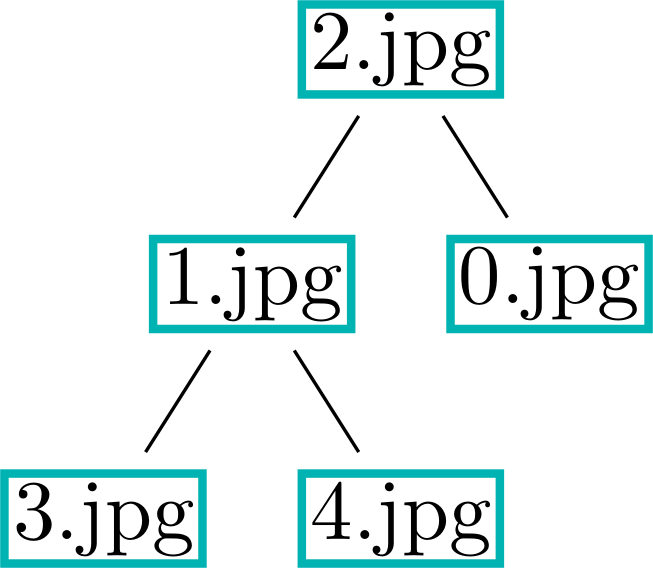
\includegraphics[width=.5\linewidth]{images/algo_tree.png}
    \caption{Arbre de phylogénie}
    \label{algo_tree}
  \end{subfigure}%
  \begin{subfigure}{.5\textwidth}
    \centering
    \begin{tabular}{|r||c|c|c|c|c|}
      \hline
      - & $I_{0}$ & $I_{1}$ & $I_{2}$ & $I_{3}$ & $I_{4}$ \\ \hhline{|=::=|=|=|=|=|}
      $I_{0}$ & - & 0 & 0 & 0 & 0 \\ \hline
      $I_{1}$ & 0 & - & 0 & 1 & 1 \\ \hline
      $I_{2}$ & 1 & 1 & - & 1 & 1 \\ \hline
      $I_{3}$ & 0 & 0 & 0 & - & 0 \\ \hline
      $I_{4}$ & 0 & 0 & 0 & 0 & - \\ \hline
    \end{tabular} 
    \caption{Matrice de parenté}
    \label{parentage_matrix}
  \end{subfigure}
  \caption{Une arbre de phylogénie et sa matrice de parenté.}
  \label{parentage_tree}
\end{figure}

Nous donnons l'algorithme de reconstruction d'arbre à titre indicatif algorithme \ref{algo_}.

\begin{algorithm}[]
  \LinesNumbered
  \KwData{M a n$\times$n parentage matrix}
  \KwResult{the root of the tree}
  \BlankLine
  $nextRoot \leftarrow$ row with min sum of elements\;
  $treeRoot \leftarrow nextRoot$\;
  \BlankLine

  \ForAll{rows row of M}{
    $root \leftarrow nextRoot$\;
    mark $root$ as done\;
    \BlankLine
    \For{$i\leftarrow 0$ \KwTo n}{
      $row[i] \leftarrow 0$\;
      \If{sum of elements of row == 0} {
        add $i$ as child of $root$\;
      }
      \If{row has the smallest sum of elements and is not marked as done} {
        $nextRoot \leftarrow i$\;
      }
    }
  }
  \KwRet treeRoot
\caption{Construction de l'arbre}
\label{algo_}
\end{algorithm}
\vspace{5mm}

À chaque itération, une image est sélectionnée comme la racine (lignes 1 et 11) et nommée $root$, elle est retirée (ligne 7) des ancêtres des autres images si c'est un ancêtre. Si ces autres images n'ont plus d'ancêtre (ligne 8), c'est que $root$ était le parent direct de l'image en train d'être traitée, cette image est donc ajoutée comme enfant de $root$ (ligne 9). La ligne 5 permet de ne traiter qu'une fois chaque image comme racine potentielle.

Cet algorithme a une complexité de $O(n^{2})$. Il y a deux boucles imbriquées, et si les sommes sont calculées une seule fois au début et mises à jour à chaque fois qu'un parent est enlevé, il n'y a pas de boucle supplémentaire augmentant la complexité.

\section{Filtrage des doublons}
\label{sec:filtrage}
Nous avons expliqué précédemment que des images avec le même historique de compression étaient identiques. Le fait qu'elles soient identiques peut fausser les métriques introduites par \citeauthornsc{dias2010first}. En effet, prenons le cas de trois images $I_m$, $I_n$ et $I_k$, où $I_m$ et $I_n$ sont identiques, et $I_k$ est l'enfant de $I_m$. Ces deux images étant identiques, $I_k$ peut aussi bien être l'enfant de $I_m$ que de $I_n$, sans que cela ne change rien aux caractéristiques de $I_k$. Mais lors de la reconstruction de l'arbre, si $I_k$ est marquée comme enfant de $I_n$, les métriques de \citeauthornsc{dias2010first} marqueront $I_k$ comme ayant le mauvais parent, et donc donneront un mauvais score à la reconstruction, alors qu'elle est fondamentalement juste. Le processus de filtrage des doublons est illustré figure \ref{fig:identique}. 

Ce filtrage est appliqué aussi bien à l'arbre original qu'à l'arbre reconstruit, pour qu'ils soient comparables.


\begin{figure}
\centering
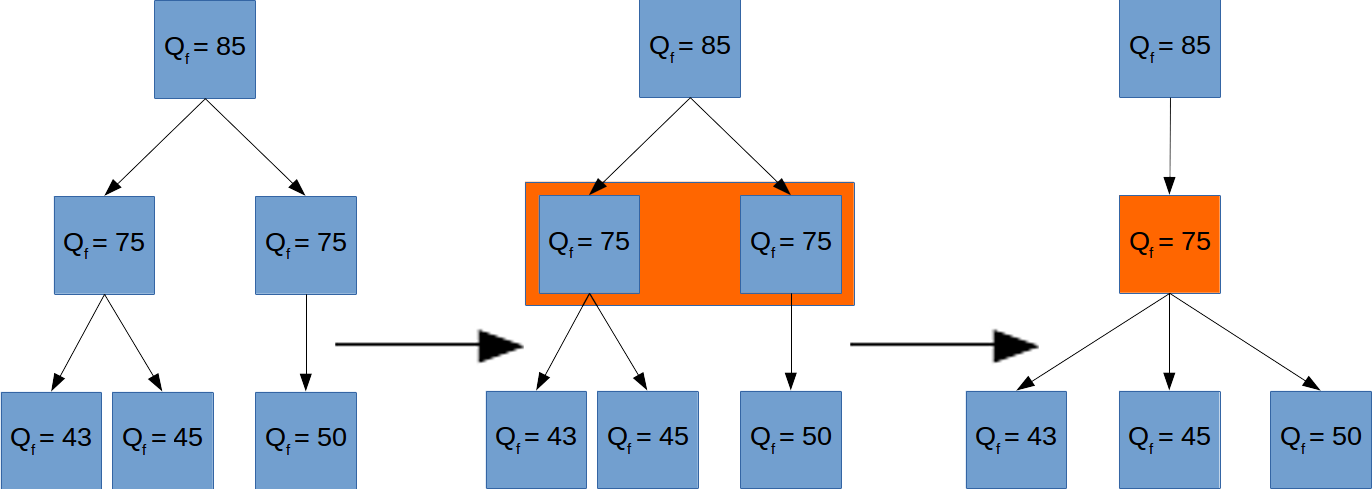
\includegraphics[width=0.9\linewidth]{images/fusion_1}
% 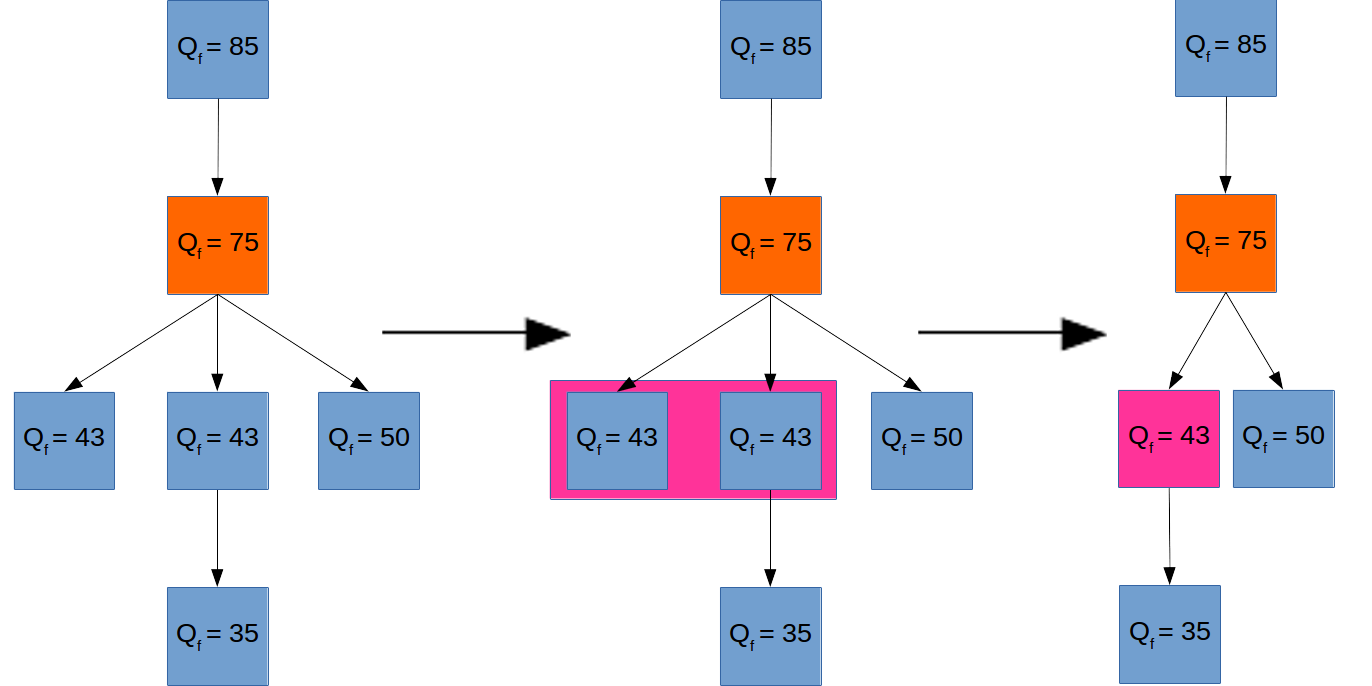
\includegraphics[width=0.9\linewidth]{images/fusion_2}
\caption{Fusion des images identiques dans l'arbre}
\label{fig:identique}
\end{figure}

% On peut voir que le seul marqueur a avoir été utilisé est le $Q_f$ de l'image. 

\chapter{Résultats}
\label{chap4}

\section{Génération des données}
Nous avons choisi de créer trois datasets différents, un avec des arbres de 15 images, un autre avec des arbres de 25 images et un dernier avec des arbres de 50 images. Cela nous permettra d'observer les différences éventuelles que peuvent amener des choses telles que la distance à la racine et le nombre de recompression dans la précision de l'estimation du parent.

La génération se fait comme suit : à partir d'une image graine (non compressée), une première image est compressée avec $85 < Q_f < 99$, c'est l'image racine. Cette image racine est ajoutée à notre pool d'images. Tant que le nombre désiré d'images n'a pas été atteint, une image est prise aléatoirement dans la pool, est compressée avec $Q_{f_{parent}} - 15 < Q_{f_{enfant}} < Q_{f_{parent}} - 1$ et est ajoutée à la pool d'image. On fixe cependant $Q_f = 30$ comme limite basse du facteur de qualité, au delà de cette limite, l'image est trop détériorée, et en plus de ne pas être un cas d'utilisation réaliste dans les réseaux sociaux, ne contient plus assez d'informations pour être correctement utilisée.

La génération des datasets en eux même est faite à partir des six images d'origine de \textit{BOWS 2}\autocite{bows} où chaque image à servi à générer 15 arbres pour chaque image pour chaque dataset, pour un total de 90 arbres par dataset, soit 8100 images tout dataset confondu.

\section{Résultats expérimentaux}

Nous allons commencer par donner le résultat de nos algorithme sur un arbre choisis aléatoirement dans notre dataset, pour bien détailler la sortie de chaque étape, puis nous allons donner des résultats plus significatifs obtenus en lançant notre programme sur l'ensemble des données.

\subsection{Détail sur un arbre}
Nous choisissons un arbre de 15 images, les résultats ne sont pas significativement différent avec les autres tailles d'arbre, et il est plus simple de tout montrer avec un nombre restreint d'images. Notons que les résultats pour cet arbre sont donnés à titre d'exemple, et ne représentent pas forcément les résultats que l'on peut obtenir sur un grand nombre d'arbre. L'image utilisée pour générer l'arbre est disponible figure \ref{casimir}

\begin{figure}
\centering
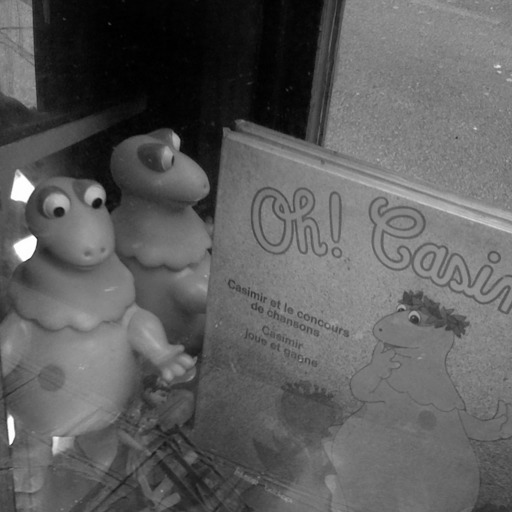
\includegraphics[width=0.5\linewidth]{images/casimir}
\caption{Image utilisée pour générer l'arbre}
\label{casimir}
\end{figure}

\paragraph{}
Commençons par la détection de pics et l'autocorrélation. Nous utilisons les 35 premiers coefficients DCT, les coefficients suivant sont trop quantifiés, et souvent à 0, et ne contiennent pas suffisamment d'informations pour être intéressants, ils peuvent même fausser les résultats. Nous donnons l'histogramme du coefficient DC ainsi que son autocorrélation figure \ref{fig:histo0}, puis le coefficient 18 dans l'ordre zigzag figure \ref{fig:histo18} et enfin le coefficent 31 figure \ref{fig:histo31} pour permettre au lecteur de visualiser les données avec lesquels nous travaillons. Ces exemples sont donnés à titre indicatif, l'apparence des histogrammes et autocorrélations peut grandement varier selon le facteur de qualité de l'image. L'image dont sont tirées les figures est compressées avec comme historique de compression $H_{Q_{f}} = \{86, 85, 73\}$. C'est la période, ou l'écart entre deux pics de l'autocorrélation de chaque coefficient DCT que nous cherchons à obtenir pour ensuite pouvoir les comparer avec les valeurs des différentes tables de quantification.

\begin{figure}
  \begin{subfigure}{.5\textwidth}
    \centering
    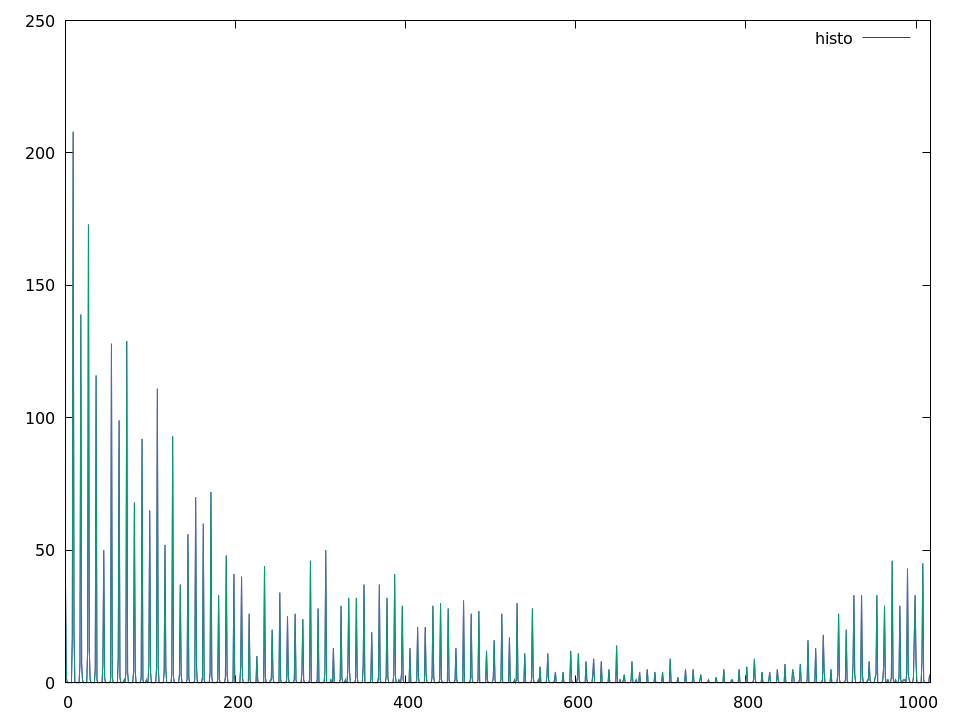
\includegraphics[width=\linewidth]{images/histos/histo0}
    \caption{Histogramme}
  \end{subfigure}
  \begin{subfigure}{.5\textwidth}
    \centering
    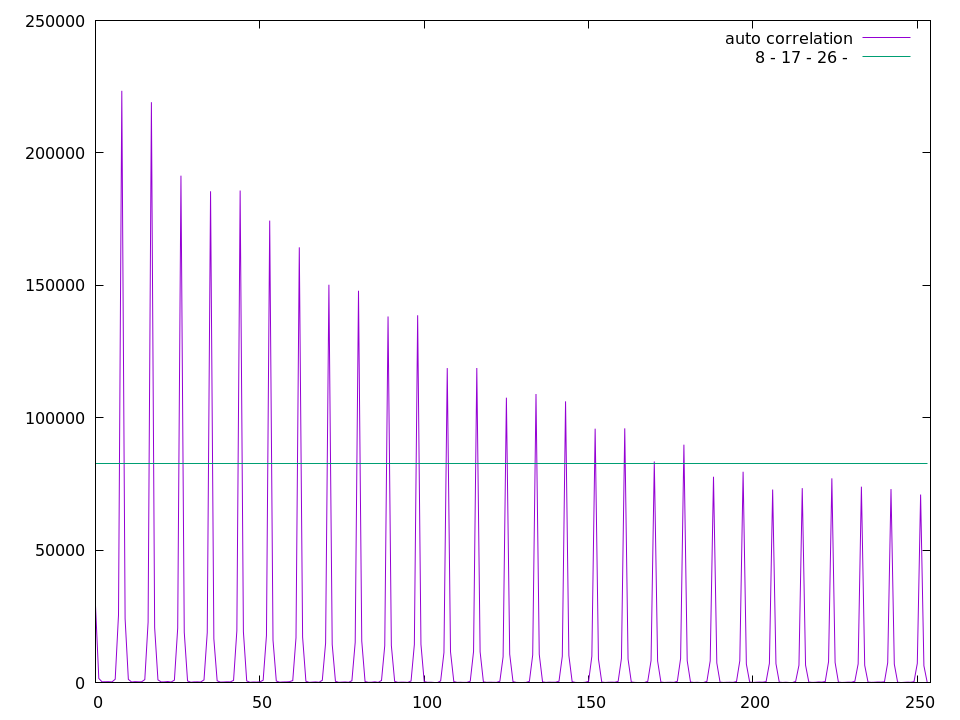
\includegraphics[width=\linewidth]{images/histos/autocorrelation0}
    \caption{Autocorrélation}
    \label{fig:histo0_auto}
  \end{subfigure}
  \caption{Histogramme et autocorrélation du coefficient DC avec figure \ref{fig:histo0_auto}, en vert le seuil et en haut à droite les pics détectés}
  \label{fig:histo0}
\end{figure}

\begin{figure}
  \begin{subfigure}{.5\textwidth}
    \centering
    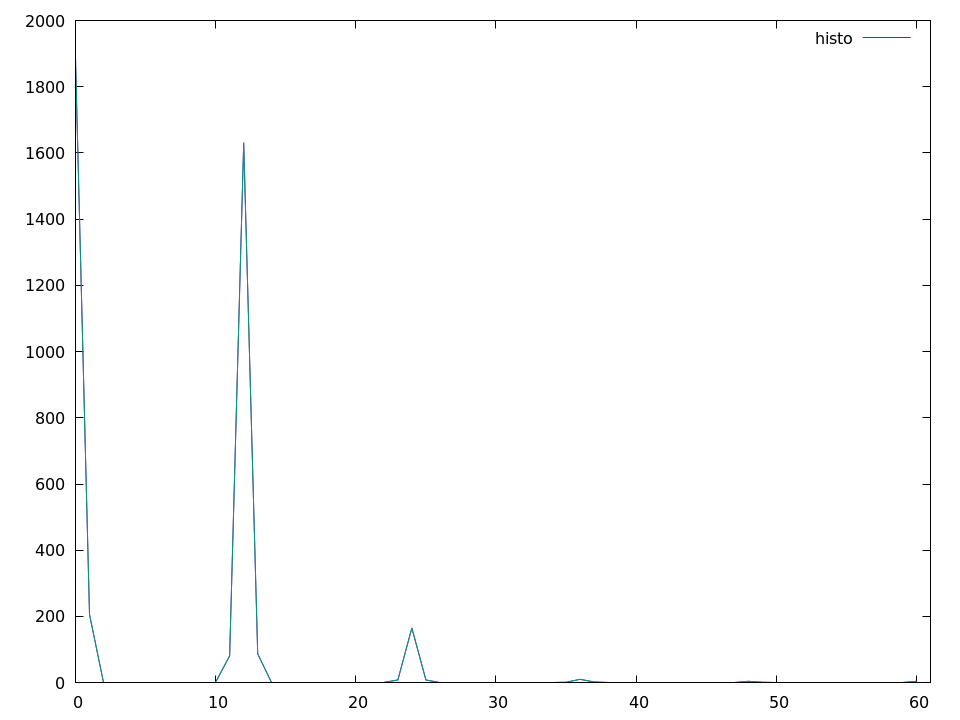
\includegraphics[width=\linewidth]{images/histos/histo18}
    \caption{Histogramme}
  \end{subfigure}
  \begin{subfigure}{.5\textwidth}
    \centering
    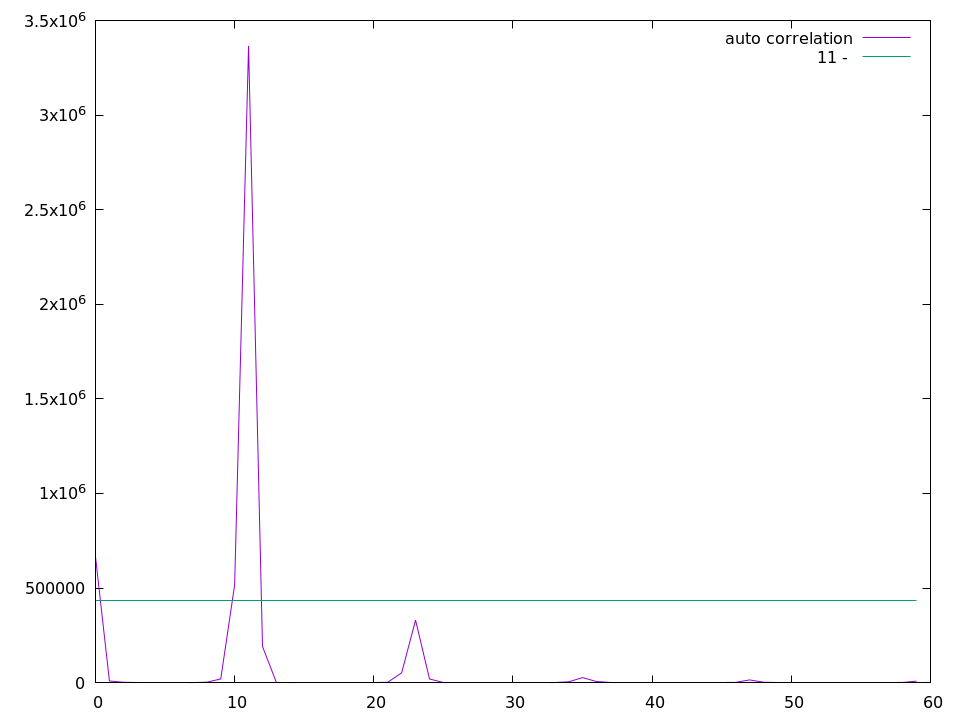
\includegraphics[width=\linewidth]{images/histos/autocorrelation18}
    \caption{Autocorrélation}
    \label{fig:histo18_auto}
  \end{subfigure}
  \caption{Histogramme et autocorrélation du 18ème coefficient AC avec figure \ref{fig:histo18_auto}, en vert le seuil et en haut à droite les pics détectés}
  \label{fig:histo18}
\end{figure}

\begin{figure}
  \begin{subfigure}{.5\textwidth}
    \centering
    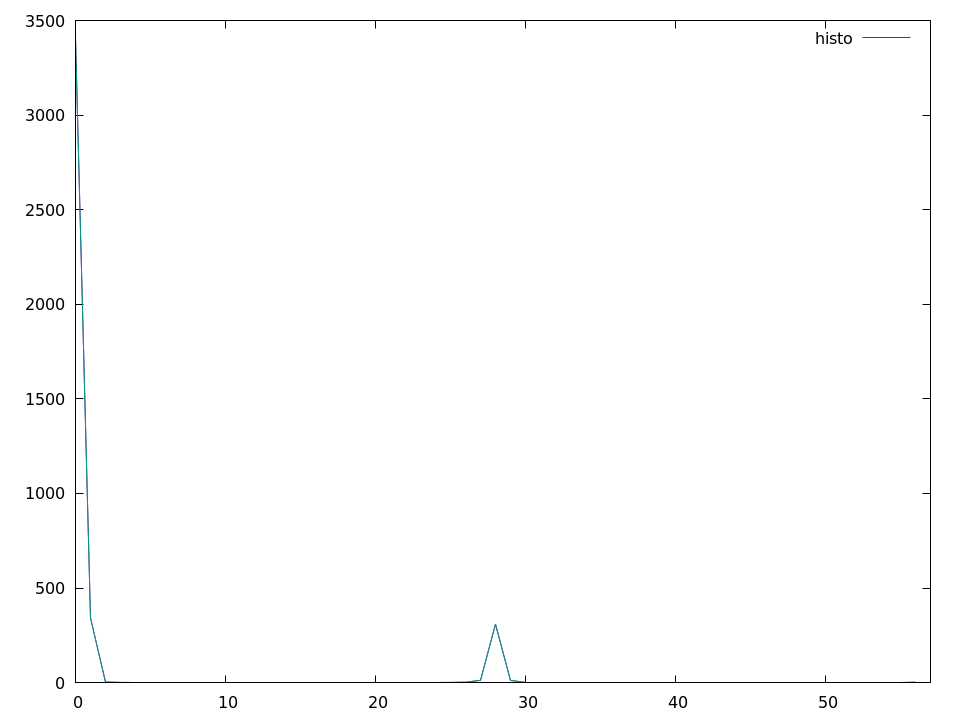
\includegraphics[width=\linewidth]{images/histos/histo31}
    \caption{Histogramme}
  \end{subfigure}
  \begin{subfigure}{.5\textwidth}
    \centering
    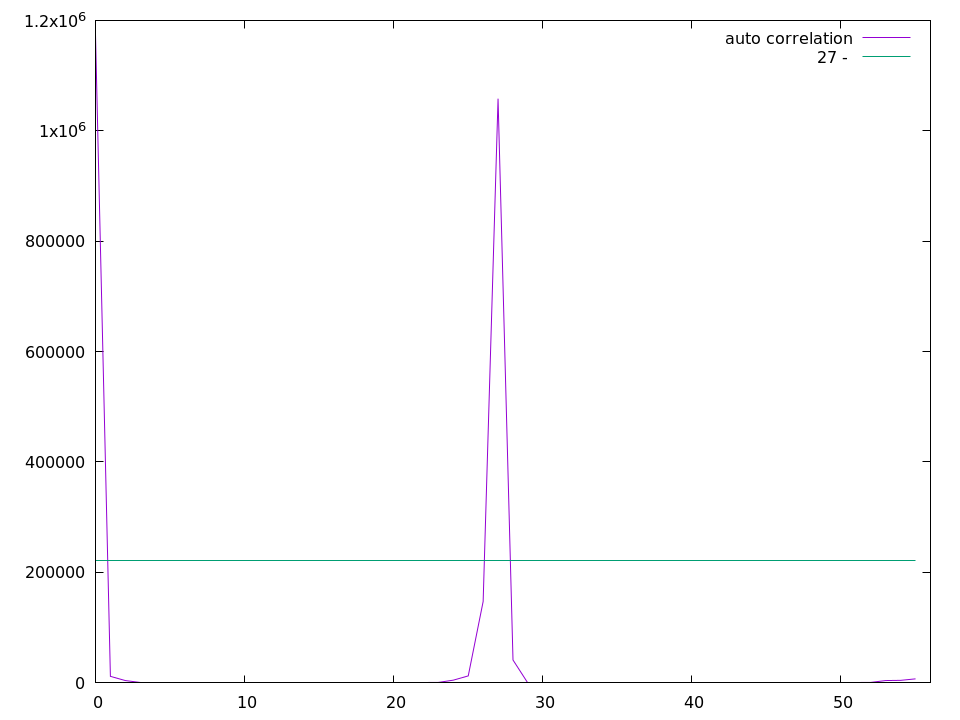
\includegraphics[width=\linewidth]{images/histos/autocorrelation31}
    \caption{Autocorrélation}
    \label{fig:histo31_auto}
  \end{subfigure}
  \caption{Histogramme et autocorrélation du 31ème coefficient AC avec figure \ref{fig:histo31_auto}, en vert le seuil et en haut à droite les pics détectés}
  \label{fig:histo31}
\end{figure}

On voit très nettement que la quantité d'information disponible baisse très fortement lorsque l'on s'éloigne du coefficient DC. C'est pour cette raison que nous restons sur 35 coefficients.

\paragraph{}
Nous allons ensuite calculer la distance entre la table de quantification $\widehat{q}(u,v)$ issues des periodes et toutes les tables de quantification de $Q_f = 1$ à $Q_f = 100$. La figure \ref{fig:distances} illustre ce calcul. Le point le plus bas de la courbe, là où la distance entre les deux tables est la plus faible est le $Q_f$ le plus probable avec lequel l'image a été compressée. Il s'agit ici de $Q_f = 71$. La table de quantification $\widehat{q}(u,v)$ est donnée table \ref{periods1}, avec pour comparaison la table de quantification d'une images compressée avec $Q_f = 71$ table \ref{periods2}, comme l'a été estimée l'image après l'estimation primaire, et la table de quantification de $Q_f = 73$ (table \ref{periods3}), le vrai $Q_f$ de l'image. Les valeurs à -1 indiquent qu'aucune valeur de période n'a pu être calculée, et sont donc ignorées, les valeurs à 0 sont celles pour lesquelles l'indice est supérieur à 35.

\begin{figure}
  \centering
  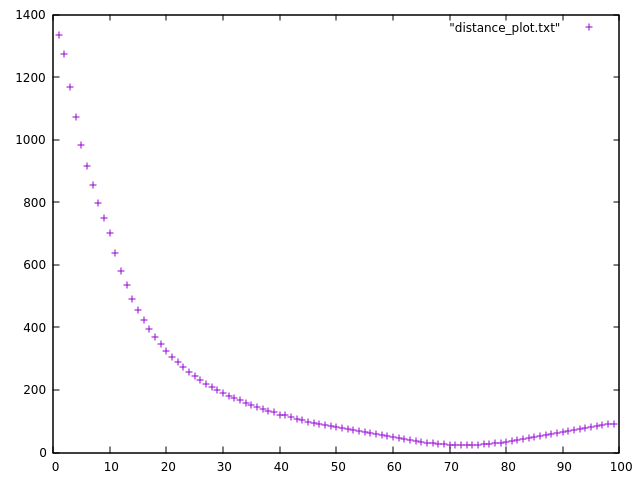
\includegraphics[width=0.7\linewidth]{images/distances}

  \caption{Distances entre la table de quantification calculée $\widehat{q}(u,v)$ et les différentes tables de quantification JPEG}
  \label{fig:distances}
\end{figure}

\begin{figure}
  \begin{subfigure}{.5\textwidth}
    \centering
    \begin{tabular}{|c|c|c|c|c|c|c|c|}
      \hline
      9 & 6 & 5 & 9 & 13 & 22 & 22 & 31 \\ \hline    
      6 & 6 & 8 & 10 & 14 & 16 & 28 & 0 \\ \hline
      8 & 7 & 9 & 13 & 20 & -1 & 0 & 0 \\ \hline
      8 & 9 & 12 & 19 & -1 & -1 & 0 & 0 \\ \hline
      10 & 12 & -1 & 31 & 30 & 0 & 0 & 0 \\ \hline
      12 & 13 & 28 & 30 & 0 & 0 & 0 & 0 \\ \hline
    \end{tabular}
    \caption{Table de quantification calculée, $\widehat{q}(u,v)$}
    \label{periods1}
  \end{subfigure}
  \begin{subfigure}{.5\textwidth}
    \centering
    \begin{tabular}{|c|c|c|c|c|c|c|c|}
      \hline
      9 & 6 & 8 & 8 & 10 & 13 & 26 & 39  \\ \hline
      6 & 6 & 7 & 9 & 12 & 19 & 35 & 50  \\ \hline
      5 & 8 & 9 & 12 & 20 & 30 & 42 & 51  \\ \hline
      9 & 10 & 13 & 16 & 30 & 35 & 47 & 53  \\ \hline
      13 & 14 & 22 & 28 & 37 & 44 & 56 & 60  \\ \hline
      22 & 31 & 31 & 47 & 59 & 56 & 65 & 54  \\ \hline
    \end{tabular}
    \caption{Table de quantification réelle, $i = 73$}
    \label{periods3}
  \end{subfigure}
\vspace{5mm}

  \begin{subfigure}{.5\textwidth}
    \centering
    \begin{tabular}{|c|c|c|c|c|c|c|c|}
      \hline
      9 & 7 & 8 & 8 & 10 & 14 & 28 & 42 \\ \hline
      6 & 7 & 8 & 10 & 13 & 20 & 37 & 53 \\ \hline
      6 & 8 & 9 & 13 & 21 & 32 & 45 & 55 \\ \hline
      9 & 11 & 14 & 17 & 32 & 37 & 50 & 57 \\ \hline
      14 & 15 & 23 & 30 & 39 & 47 & 60 & 65 \\ \hline
      23 & 34 & 33 & 50 & 63 & 60 & 70 & 58 \\ \hline
    \end{tabular}
    \caption{Table de quantification estimée, distance entre $\widehat{q}(u,v)$ et table(i) la plus faible, $i = 71$}
    \label{periods2}
  \end{subfigure}

% \caption{Tables de quantifications }
\end{figure}

\paragraph{}
Toutes les images de l'arbre subiront l'estimation primaire de la même manière pour obtenir $Q_f$, puis l'estimation secondaire grâce aux formules \ref{eqn:jpeg_1} et \ref{eqn:jpeg_2} affinera les résultats. La table \ref{rough_fine} montre les résultats de l'estimation primaire puis de l'estimation secondaire en donnant également leur véritable $Q_f$ comme comparaison et la différence entre l'estimation primaire et les valeurs réelles et la différence entre l'estimation secondaire et les valeurs réelles pour pouvoir les comparer. On peut voir que l'estimation secondaire est strictement meilleure que l'estimation primaire, ce qui ne se limite pas à ce cas précis, mais s'est vérifié de manière expérimentale sur toutes les estimations. L'erreur moyenne d'estimation de la table \ref{rough_fine} est de $0.533333$.

\begin{figure}
  \begin{tabular}{|l||c|c|c|c|c|c|c|c|c|c|c|c|c|c|c|}
    \hline
    Image & $I_{0}$ & $I_{1}$ & $I_{2}$ & $I_{3}$ & $I_{4}$ & $I_{5}$ & $I_{6}$ & $I_{7}$ & $I_{8}$ & $I_{9}$ & $I_{10}$ & $I_{11}$ & $I_{12}$ & $I_{13}$ & $I_{14}$ \\ \hhline{|=::=|=|=|=|=|=|=|=|=|=|=|=|=|=|=|}
   
    \textbf{Primaire}  & 71 & 81 & 71 & 58 & 78 & 46 & 61 & 85 & 81 & 79 & 65 & 74 & 84 & 71 & 74 \\ \hline
    \textbf{Secondaire} & 71 & 81 & 71 & 58 & 78 & 46 & 61 & 87 & 82 & 80 & 65 & 74 & 85 & 71 & 75 \\ \hline
    \textbf{Valeurs réelles} & 73 & 81 & 71 & 57 & 79 & 44 & 62 & 86 & 82 & 80 & 65 & 74 & 85 & 71 & 75 \\ \hhline{|=::=|=|=|=|=|=|=|=|=|=|=|=|=|=|=|}
    \textbf{Delta primaire} & -2 & 0 & 0 & 1 & -1 & 2 & -1 & -1 & -1 & -1 & -1 & 0 & -1 & 0 & -1 \\ \hline
    \textbf{Delta secondaire} & -2 & 0 & 0 & 1 & -1 & 2 & -1 & 1 & 0 & 0 & 0 & 0 & 0 & 0 & 0 \\ \hline
  \end{tabular}

  \caption{Estimations primaires et secondaires des $Q_f$ des images de l'arbre}
  \label{rough_fine}
\end{figure}

\paragraph{}
Ces $Q_f$ vont ensuite servir à compresser les images pour pouvoir les comparer deux à deux, il semble peu intéressant de détailler les calculs qui sont effectués, aussi nous nous contenterons de donner la matrice de parenté (figure \ref{parentage_matrix_example}) produite en sortie. L'arbre calculé à partir de cette matrice (figure \ref{tree_example}) est exactement identique à l'arbre original.

\begin{figure}
  \centering
  \begin{tabular}{|c||c|c|c|c|c|c|c|c|c|c|c|c|c|c|c|}
    \hline
    - & $I_{0}$ & $I_{1}$ & $I_{2}$ & $I_{3}$ & $I_{4}$ & $I_{5}$ & $I_{6}$ & $I_{7}$ & $I_{8}$ & $I_{9}$ & $I_{10}$ & $I_{11}$ & $I_{12}$ & $I_{13}$ & $I_{14}$ \\ \hhline{|=::=|=|=|=|=|=|=|=|=|=|=|=|=|=|=|}
    $I_{0}$ & - & 0 & 0 & 0 & 0 & 0 & 0 & 0 & 0 & 0 & 0 & 0 & 1 & 0 & 0 \\ \hline 
    $I_{1}$ & 0 & - & 0 & 0 & 0 & 0 & 0 & 0 & 1 & 0 & 0 & 0 & 0 & 0 & 0 \\ \hline 
    $I_{2}$ & 0 & 0 & - & 0 & 0 & 0 & 0 & 0 & 0 & 0 & 0 & 0 & 1 & 0 & 0 \\ \hline 
    $I_{3}$ & 0 & 0 & 0 & - & 0 & 0 & 0 & 0 & 0 & 0 & 0 & 0 & 0 & 1 & 0 \\ \hline 
    $I_{4}$ & 0 & 0 & 0 & 0 & - & 0 & 0 & 0 & 0 & 0 & 0 & 0 & 1 & 0 & 0 \\ \hline 
    $I_{5}$ & 0 & 0 & 0 & 1 & 0 & - & 0 & 0 & 0 & 0 & 0 & 0 & 0 & 0 & 0 \\ \hline 
    $I_{6}$ & 0 & 0 & 0 & 0 & 0 & 0 & - & 0 & 0 & 0 & 1 & 0 & 0 & 0 & 0 \\ \hline 
    $I_{7}$ & 0 & 0 & 0 & 0 & 0 & 0 & 0 & - & 0 & 0 & 0 & 0 & 0 & 0 & 0 \\ \hline 
    $I_{8}$ & 0 & 0 & 0 & 0 & 0 & 0 & 0 & 1 & - & 0 & 0 & 0 & 0 & 0 & 0 \\ \hline 
    $I_{9}$ & 0 & 1 & 0 & 0 & 0 & 0 & 0 & 0 & 0 & - & 0 & 0 & 0 & 0 & 0 \\ \hline 
    $I_{10}$& 0 & 0 & 0 & 0 & 0 & 0 & 0 & 0 & 0 & 0 & - & 0 & 0 & 1 & 0 \\ \hline 
    $I_{11}$& 0 & 0 & 0 & 0 & 0 & 0 & 0 & 1 & 0 & 0 & 0 & - & 0 & 0 & 0 \\ \hline 
    $I_{12}$& 0 & 0 & 0 & 0 & 0 & 0 & 0 & 1 & 0 & 0 & 0 & 0 & - & 0 & 0 \\ \hline 
    $I_{13}$& 0 & 0 & 0 & 0 & 0 & 0 & 0 & 0 & 1 & 0 & 0 & 0 & 0 & - & 0 \\ \hline 
    $I_{14}$& 0 & 0 & 0 & 0 & 0 & 0 & 0 & 0 & 0 & 1 & 0 & 0 & 0 & 0 & - \\ \hline 

  \end{tabular}
  \caption{Matrice de parenté}
  \label{parentage_matrix_example}
\end{figure}

\begin{figure}[H]
  \begin{subfigure}{.5\textwidth}
    \centering
    \scalebox{0.85}{
      \begin{forest}
        [\href{run:7.jpg}{7.jpg}[\href{run:8.jpg}{8.jpg}[\href{run:13.jpg}{13.jpg}[\href{run:3.jpg}{3.jpg}[\href{run:5.jpg}{5.jpg}]][\href{run:10.jpg}{10.jpg}[\href{run:6.jpg}{6.jpg}]]][\href{run:1.jpg}{1.jpg}[\href{run:9.jpg}{9.jpg}[\href{run:14.jpg}{14.jpg}]]]][\href{run:12.jpg}{12.jpg}[\href{run:2.jpg}{2.jpg}][\href{run:4.jpg}{4.jpg}][\href{run:0.jpg}{0.jpg}]][\href{run:11.jpg}{11.jpg}]]
      \end{forest}}
    \caption{Arbre phylogénétique original}
    \label{tree_base_example}
  \end{subfigure}
  \begin{subfigure}{.5\textwidth}
    \centering
    \scalebox{0.85}{
      \begin{forest}
        [\href{run:7}{7.jpg}[\href{run:8}{8.jpg}[\href{run:1}{1.jpg}[\href{run:9}{9.jpg}[\href{run:14}{14.jpg}]]][\href{run:13}{13.jpg}[\href{run:3}{3.jpg}[\href{run:5}{5.jpg}]][\href{run:10}{10.jpg}[\href{run:6}{6.jpg}]]]][\href{run:11}{11.jpg}][\href{run:12}{12.jpg}[\href{run:0}{0.jpg}][\href{run:2}{2.jpg}][\href{run:4}{4.jpg}]]]
      \end{forest}}
    \caption{Arbre phylogénétique reconstruit}
    % \label{tree_example}
  \end{subfigure}
  \caption{Exemple d'arbre original et d'arbre reconstruit}
  \label{tree_example}
\end{figure}

\begin{figure}
  \scalebox{1.8}{
    \begin{tikzpicture}
      \node[anchor=south west,inner sep=1] at (0,0) { 
        \begin{forest}
          [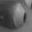
\includegraphics{images/tree/7.png}[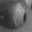
\includegraphics{images/tree/8.png}[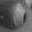
\includegraphics{images/tree/13.png}[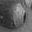
\includegraphics{images/tree/3.png}[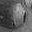
\includegraphics{images/tree/5.png}]][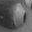
\includegraphics{images/tree/10.png}[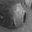
\includegraphics{images/tree/6.png}]]][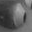
\includegraphics{images/tree/1.png}[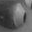
\includegraphics{images/tree/9.png}[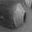
\includegraphics{images/tree/14.png}]]]][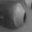
\includegraphics{images/tree/12.png}[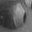
\includegraphics{images/tree/2.png}][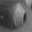
\includegraphics{images/tree/4.png}][\includegraphics{images/tree/0.png}]][\includegraphics{images/tree/11.png}]]
        \end{forest}};
    \end{tikzpicture}}
  \caption{Arbre original (figure \ref{tree_base_example}) où les noms des images ont été remplacés par leurs images, zoom sur l'oeil de Casimir}
  \label{tree_casimir}
\end{figure}

On voit qu'il y a au maximum un seul 1 par ligne dans la matrice de parenté. En effet, seuls les parents directs sont détectés, et pas les ancêtres plus éloignés. La figure \ref{tree_casimir} permet de voir la différence de qualité entre les images de l'arbre. Des imagettes de $32\times32$ représentent les images originale (de $512\times512$) pour que les artefacts JPEG soient visibles.
\subsection{Résultats sur les datasets}
Nous avons fait tourner notre collection d'algorithmes sur les trois datasets, et avons obtenu des résultats très satisfaisants. Nous mesurons la qualité de nos résultats grâce à sept métriques, trois servant à mesurer la précision de l'estimation du facteur de qualité et les quatre autres servant à mesurer la qualité du calcul de l'arbre sont celles introduites par \citeauthornsc{dias2012image} \cite{dias2012image}.

Les trois métriques servant à mesurer la précision de l'estimation du $Q_f$ sont l'erreur moyenne d'estimation, qui servira à savoir si l'estimation est juste la plupart du temps, la sur-estimation moyenne et la sous-estimation moyenne, qui, si tout va bien, seront symétriques, et serviront à savoir si notre algorithme a plutôt tendance à sur-estimer ou sous-estimer $Q_f$, et dans quel cas.

\begin{figure}[H]
  \centering
  \begin{tabular}{|l||c|c|c|c|c|}
    \hline
     \backslashbox{Métrique}{Dataset}             & \textbf{15 images} & \textbf{25 images} & \textbf{50 images} \\ \hhline{|=::=|=|=|}
    \textbf{\pbox{3.6cm}{Erreur moyenne d'estimation de $Q_f$}}         & 0.516667 & 0.639444 & 0.833333 \\ \hline
    \textbf{\pbox{3.6cm}{Sur-estimation moyenne de $Q_f$}} & 1.61111  & 1.86111  & 1.94444  \\ \hline
    \textbf{\pbox{3.6cm}{Sous-estimation moyenne de $Q_f$}}  & 1.06944  & 2.125    & 6.68056  \\ \hhline{|=::=|=|=|}
    \textbf{roots}              & 0.958333 & 0.888889 & 0.847222 \\ \hline
    \textbf{edges}              & 0.997024 & 0.992477 & 0.989796 \\ \hline
    \textbf{leaves}             & 0.995949 & 0.991517 & 0.987451 \\ \hline
    \textbf{ancestry}           & 0.994444 & 0.968889 & 0.969699 \\ \hline
  \end{tabular} 
\caption{Table de résultats, les trois premières lignes mesurent la précision de l'estimation de $Q_f$, les autres lignes mesure la qualité de la reconstruction de l'arbre et sont données en pourcentage}
\label{results}
\end{figure}

La table \ref{results} montre les résultats obtenus par nos algorithmes. On peut directement remarquer que les résultats sont strictement meilleurs lorsque l'on réduit le nombre d'images dans le set. À noter que le meilleur résultat possible pour les trois premières métriques est zéro, c'est à dire que tout les $Q_f$ ont été estimés parfaitement, et que le meilleur résultat pour les quatre dernières est un, lorsque la vérité terrain et l'arbre reconstruit sont identiques.
\paragraph{}

Il semble important de préciser que l'estimation du $Q_f$ rencontre des difficultés lorsque $Q_f$ est proche de 100. En effet un grand nombre des valeurs de la table de quantification est à 1 ou 2, ce qui ne quantifie pas ou pas suffisamment le coefficient DCT pour que nous puissions extraire suffisamment d'information pour discriminer une image compressée avec $Q_f = 97$ d'une image compressée avec $Q_f = 99$ par exemple. C'est en partie une des causes du manque de précision d'identification de la racine. En effet, dans notre cas d'étude, la racine est l'image avec le $Q_f$ le plus proche de 100, il est difficile de l'identifier avec certitude lorsque l'estimation du $Q_f$ n'est pas certaine.

\paragraph{}
On voit que les erreurs moyennes, même si elles restent inférieures à 1 pour les trois datasets, et sont donc tout à fait correctes, sont de moins en moins bonnes lorsque le nombre d'images augmente, avec notamment la sur-estimation moyenne qui est très importante pour le dataset de 50 images.

Une telle sur-estimation s'explique par le fait que les coefficients DCT deviennent trop bruités pour pouvoir correctement estimer la période lorsqu'ils ont été compressés un trop grand nombre de fois, le signal n'est plus périodique et l'autocorrélation ne montre pas de pics. Lorsqu'aucun pic n'est détecté, notre algorithme estime que l'image a un $Q_f$ élevé, ce qui fausse la reconstruction de l'arbre, car dans notre cas, une image ayant subi un grand nombre de recompressions a forcément un $Q_f$ petit. C'est une autre source d'erreurs dans l'estimation de la racine. Plus l'arbre est grand, plus les images ont été compressées un nombre important de fois, et donc plus elles ont de chance de pouvoir fausser les résultats. Le problème vient de notre algorithme de recontruction d'arbre. Une image est marquée comme la racine si elle n'a aucun parent. La racine n'a effectivement aucun parent, mais une image ayant eu son $Q_f$ mal estimé n'aura aucun parent \textbf{détecté}. Il devient dans ce cas difficile de savoir la quelle des deux est la vraie racine.
\paragraph{}

Nous avions considéré que deux images avec le même historique de compression étaient identiques, il semble cependant que les images ayant un petit $Q_f$ (inférieur à 35 environ) échappent parfois à ce phénomène, une image parent compressée avec le $Q_f$ de son enfant et son enfant sont parfois différentes, sans que nous ayons pu identifier la cause de ce problème.
\paragraph{}

Un autre problème, qui lui n'affecte pas la racine, mais plutôt le reste de l'arbre, est la convergence des blocs, comme expliqué chapitre \ref{chap2} section \ref{convergence}. Nous avons fixé comme limite basse pour la génération de l'arbre $Q_f = 30$, si une image avec $Q_f = 30$ a un enfant, cet enfant aura également $Q_f = 30$, et ce de manière récursive. On peut donc arriver dans le cas où les enfants sont identiques à leurs parents, ce qui rend impossible leur différenciation, ce phénomène est fort heureusement assez rare.

\paragraph{}

Les résultats donnés précédemment sont obtenus en ayant la totalité de l'arbre. Notre méthode étant très efficace pour reconstruire l'arbre lorsque toutes les images sont présentes, et donc lorsqu'il y a à chaque fois un parent direct, il nous a semblé important de tester le cas où l'arbre est incomplet. Aussi, la table \ref{results_missing} montre les résultats obtenus en ayant enlevé au hasard une des images du set. Notre méthode n'étant pas en mesure d'estimer les grands-parents, nous nous retrouvons dans le cas illustré figure \ref{fig:missing}, où nous avons des arbres correctement reconstruits, sans que nous sachions comment les relier entre eux. C'est là la limite de notre méthode de reconstruction d'arbre, une fois que la matrice de parenté a été calculée, si elle est incomplete, c'est la racine des sous arbres avec le plus petit indice qui va être choisie comme racine de l'arbre reconstruit, comme on peut le voir figure \ref{fig:missing1} où c'est l'image 1 qui a été choisie comme racine. Les résultats table \ref{results_missing} montrent clairement le phénomène expliqué précédemment, le score de détection de la racine chute drastiquement, alors que les autres métriques, bien que logiquement moins bonnes, restent tout à fait correctes.

\begin{figure}
  \begin{subfigure}{.5\textwidth}
    \centering
    \begin{tikzpicture}
      \node[anchor=south west,inner sep=2] at (0,0) { 
        \begin{forest}
          [\href{run:7}{7.jpg}[\href{run:8}{8.jpg}[\href{run:1}{1.jpg}[\href{run:9}{9.jpg}[\href{run:14}{14.jpg}]]][\href{run:13}{13.jpg}[\href{run:3}{3.jpg}[\href{run:5}{5.jpg}]][\href{run:10}{10.jpg}[\href{run:6}{6.jpg}]]]][\href{run:11}{11.jpg}][\href{run:12}{12.jpg}[\href{run:0}{0.jpg}][\href{run:2}{2.jpg}][\href{run:4}{4.jpg}]]]
        \end{forest}};
      % \draw[red,ultra thick,rounded corners] (7.5,5.3) rectangle (9.4,6.2);
      \draw[red, ultra thick](1,2.7) -- (2.2,3.3);
      \draw[red, ultra thick](1,3.3) -- (2.2,2.7);
    \end{tikzpicture}
    \caption{Arbre original avec le noeud 8 retiré}
  \end{subfigure}
  \begin{subfigure}{.5\textwidth}
    \centering
    \begin{tikzpicture}
      \node[anchor=south west,inner sep=2] at (0,0) { 
        \begin{forest}
          [\href{run:7}{7.jpg}[\href{run:11}{11.jpg}][\href{run:12}{12.jpg}[\href{run:0}{0.jpg}][\href{run:2}{2.jpg}][\href{run:4}{4.jpg}]]]
        \end{forest}
        \begin{forest}
          [\href{run:1}{1.jpg}[\href{run:9}{9.jpg}[\href{run:14}{14.jpg}]]]
        \end{forest}
        \begin{forest}
          [\href{run:13}{13.jpg}[\href{run:3}{3.jpg}[\href{run:5}{5.jpg}]][\href{run:10}{10.jpg}[\href{run:6}{6.jpg}]]]
        \end{forest}};
    \end{tikzpicture}
    \caption{Trois sous arbre que l'on se sait pas comment relier}
  \end{subfigure}

  \begin{subfigure}{.5\textwidth}
    \centering
    \begin{forest}
      [\href{run:1}{1.jpg}[\href{run:7}{7.jpg}[\href{run:11}{11.jpg}][\href{run:12}{12.jpg}[\href{run:0}{0.jpg}][\href{run:2}{2.jpg}][\href{run:4}{4.jpg}]]][\href{run:9}{9.jpg}[\href{run:14}{14.jpg}]][\href{run:13}{13.jpg}[\href{run:3}{3.jpg}[\href{run:5}{5.jpg}]][\href{run:10}{10.jpg}[\href{run:6}{6.jpg}]]]]
    \end{forest}
    \caption{Arbre reconstruit avec l'image 8 manquante}
    \label{fig:missing1}
  \end{subfigure}

  \caption{Exemple de cas où un noeud est enlevé et où l'on ne sait pas comment reconstruire}
  \label{fig:missing}
\end{figure}

\begin{figure}[H]
  \centering
  \begin{tabular}{|l||c|c|c|c|c|}
    \hline
     \backslashbox{Métrique}{Dataset}             & \textbf{15 images} & \textbf{25 images} & \textbf{50 images} \\ \hhline{|=::=|=|=|}
    \textbf{roots}                                                      & 0.696078 & 0.333333 & 0.490196 \\ \hline
    \textbf{edges}                                                      & 0.888655 & 0.924019 & 0.95078  \\ \hline
    \textbf{leaves}                                                     & 0.913087 & 0.930065 & 0.947263 \\ \hline
    \textbf{ancestry}                                                   & 0.780631 & 0.822239 & 0.882112 \\ \hline
  \end{tabular} 
\caption{Table de résultats des datasets avec une image manquante}
\label{results_missing}
\end{figure}

\chapter{Perspectives et conclusion}
\label{chap5}
Au terme de cette étude, nous avons pu voir que le problème de la reconstruction d'arbre phylogénétique d'images dans les réseaux sociaux n'est pas trivial et peut se diviser en deux sous-parties : l'identification de la racine et l'estimation des relations parent-enfant. Nous avons également pu voir dans l'état de l'art les différentes approches de reconstruction d'arbre de phylogénie. Nous avons choisi de nous concentrer uniquement sur l'étude des recompressions JPEG pour le calcul de l'arbre. Cette décision est motivée par le fait que nous sommes intéressés par le domaine du forensics et que l'étude des recompressions un sujet suffisamment vaste et complexe. Cela nous a amené à étudier la détection des compressions multiples.

De cette étude nous avons formalisé un théorème et réduit la reconstruction de l'arbre à une décision binaire entre deux images. Nous avons également précisément identifié les buts à atteindre dans la suite de ce stage : identifier une fonction qui trouve, s'il est présent, un marqueur qui prouve qu'il n'y a pas de relation parent-enfant entre deux images.


% \nocite{*}
\printbibliography

\end{document}

    
%%% Local Variables: 
%%% mode: latex
%%% TeX-master: t
%%% End:  
 